\makeatletter
\def\input@path{{../}}
\makeatother

\documentclass[/main.tex]{subfiles}
\graphicspath{{./pics/}{ch4/pics/}}
\begin{document}

\onlyinsubfile{\textpages}
\chapter{Searching for Double Beta Decay to Excited States}

\section{Introduction}

\Se{76} has 3 excited states that \Ge{76} can decay into in addition to the ground state, as shown in figure~\ref{fig:Ge76BBLevelDiagram}.
While the ground state decay has been observed, none of the decays to excited states have been yet; current experimental limits and theoretical estimates for the half-life of each decay are listed in table~\ref{tab:Ge76HalfLives}.
Each excited state decay will have a \bb -decay with a reduced \Qval\ compared to the ground state decay.
The excited state decays will also promptly produce one or two $\gamma$-rays at known energies.
These $\gamma$s will typically travel several cms before absorption and will often hit a different detector from the \bb -decay site, meaning that we can search for peaks at these energies.
\\
\begin{figure}[h]
  \centering
  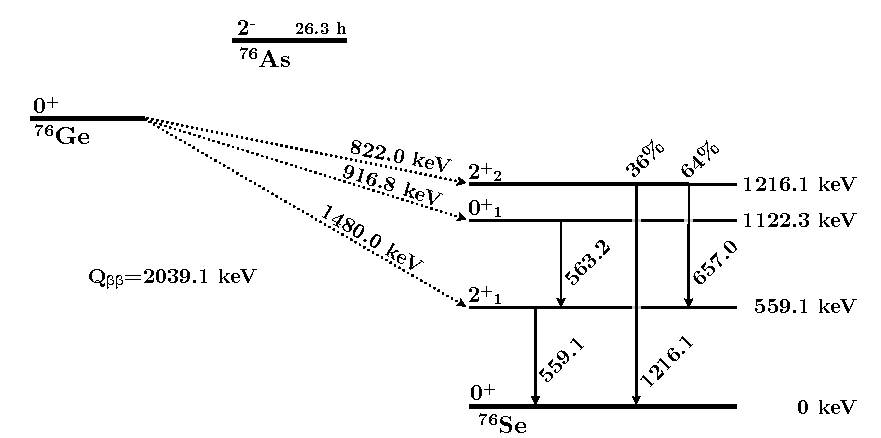
\includegraphics[width=0.8\textwidth]{leveldiagram}
  \caption[Energy level diagram for \Ge{76} \bb to \Se{76}]{\label{fig:Ge76BBLevelDiagram}
    Energy level diagram for \bb-decay of \Ge{76} to \Se{76}, including excited states. The \Qval s for each decay branch and the energies and branching ratios for the deexcitation $\gamma$s are shown next to their corresponding lines.}
\end{figure}

\begin{table}[p]
  \caption[Current half-live limits and predictions for all \tnbb-decay modes of \Ge{76}]{\label{tab:Ge76HalfLives}
    Table of best experimental limits and theoretical predictions for the half-life of each each \Ge{76}\ \bbes\ decay mode.
  }
  \begin{tabu}{|[2pt]c|r|c c c|[2pt]}
  \hlinethick
  \tnbb\ Decay Mode & \hl{2\nu\beta\beta}~(yr) & Experiment/Model & ref. & year \\
  \hlinethick
  \multirow{2}{*}{\makecell{\gs -- \gs \\ \Qbb$=2039$~keV}}
  & $(1.926 \pm 0.094)\e{21}$& \Gerda\ Phase I & \cite{Agostini:2015nwa} & 2015 \\
  & & \MJD & & \\
  \hlinethick
  \multirow{9}{*}{\makecell{\gs -- \SP{0}{+}{1} \\ \Qbb$=916.8$~keV \\ $559.1 + 563.2$~keV~$\gamma$}}
  & $>3.7\e{23}$ & \Gerda\ Phase I & \cite{Agostini_2015} & 2015 \\
  \cline{2-5}
  & $1.32\e{21}$ & HFB & \cite{PhysRevC.50.R2660} & 1994 \\
  & $4.0\e{22}$ & QRPA & \cite{} & 1994 \\
  & $4.5\e{22}$ & QRPA & \cite{} & 1996 \\
  & $7.5\e{21}$ & MCM-QRPA & \cite{} & 1996 \\
  & $(1.0-3.1)\e{23}$ & RQRPA & \cite{} & 1997 \\
  & $(1.2-5.8)\e{23}$ & RQRPA & \cite{} & 2014 \\
  & $6.4\e{24}$ & IBM-2 & \cite{} & 2014 \\
  & $(2.3-6.7)\e{24}$ & SM & \cite{} & 2014 \\
  \hlinethick
  \multirow{9}{*}{\makecell{\gs -- \SP{2}{+}{1} \\ \Qbb$=1480.0$~keV \\ $559.1$~keV~$\gamma$}}
  & $>1.6\e{23}$ & \Gerda\ Phase I & \cite{Agostini_2015} & 2015 \\
  \cline{2-5}
  & $1.2\e{30}$ & SM & \cite{} & 1984 \\
  & $5.8\e{23}$ & HFB & \cite{} & 1994 \\
  & $5.0\e{26}$ & QRPA & \cite{} & 1994 \\
  & $2.4\e{24}$ & QRPA & \cite{} & 1996 \\
  & $7.8\e{25}$ & MCM-QRPA & \cite{} & 1996 \\
  & $1.0\e{26}$ & RQRPA & \cite{} & 1997 \\
  & $(2.4-4.3)\e{26}$ & RQRPA & \cite{} & 1998 \\
  & $5.75\e{28}$ & pnQRPA & \cite{} & 2007 \\
  & $2.0\e{27}$ & RQRPA & \cite{} & 2014 \\
  \hlinethick
  \multirow{4}{*}{\makecell{\gs -- \SP{2}{+}{2} \\ \Qbb$=822.0$~keV \\ $64\%: 657.0+559.1$~keV~$\gamma$ \\ $36\%: 1216.1$~keV~$\gamma$}}
  & $>2.3\e{23}$ & \Gerda\ Phase I & \cite{Agostini_2015} & 2015 \\
  \cline{2-5}
  & $1.0\e{29}$ & QRPA & \cite{} & 1994 \\
  & $1.3\e{29}$ & MCM-QRPA & \cite{} & 1996 \\
  & $(0.7-2.2)\e{28}$ & MCM-QRPA & \cite{} & 1997 \\
  \hlinethick
  
\end{tabu}

\end{table}

Furthermore, since these $gamma$s hit separate detectors, this signal is inherently \msmd.
As shown in figure~\ref{fig:multhist}, by searching for the peak only in events with high hit multiplicity, i.e. events that involve 2 or more detectors hit, $\sim85\%$ of backgrounds can be cut, while only sacrificing $\sim25$\% of the signal.
Furthermore, the coincident detector hit(s) can provide additional observables that can be used to further discriminate excited state signals from multi-site backgrounds.
This chapter will describe the various background reduction data cuts and how they are implemented.
It will also evaluate the detection efficiency and systematic error associated with each cut based on simulations of the \MJD.

\begin{figure}[h]
  \centering
  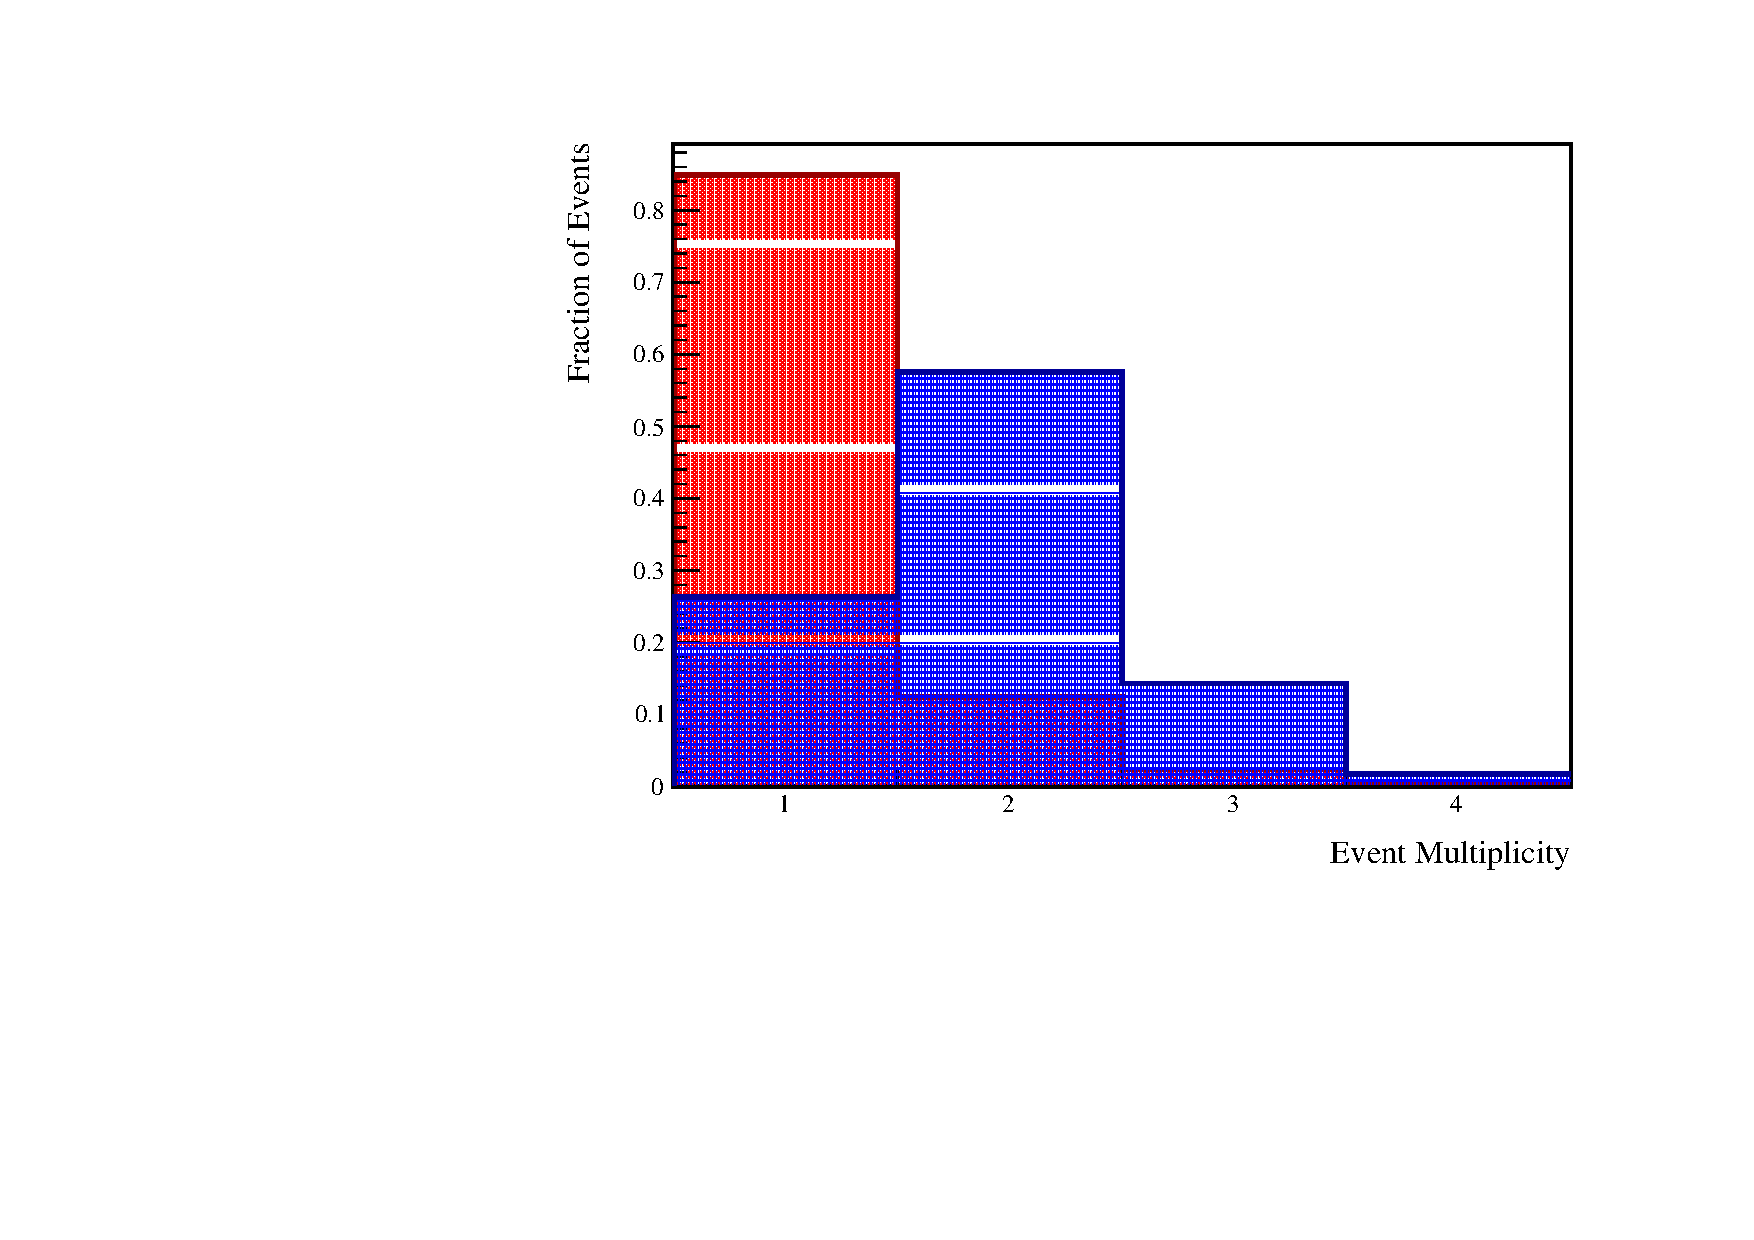
\includegraphics[width=0.8\textwidth]{MultHist}
  \caption[Event Multiplicity in E.S. decay and BG model simulations]{\label{fig:multhist}
    The simulated distribution of ROI event multiplicities in the background model and \bbes to \SP{0}{+}{1} decay. These simulations use the DS6 detector configuration.}
\end{figure}


\section{\Md s Selection}
Simultaneous detector hits are combined into events by the event builder (see section~\ref{sec:eventbuilder} and appendix~{app:eventbuilder}).
Events are combined in a 4~$\mu$s rolling window.
This window is expected to accept virtually all true coincidence events (see figure~\ref{fig:toffset}.
In a small number of runs, clocks between different Gretina cards were desyncronized.
For these runs, the clocks were resynchronized by applying a timing offset during event building that is measured by seeking the time offset that aligns pulser events.
With a typical overall rate between both modules of $<1$~Hz, $<.4\%$ of all multi-site events are expected to originate from accidental coincidence, making this a negligible background.
Once all the data has gone through the processing chain described in section~\ref{sec:datachain}, the skim files from all good runs in datasets 1\-6a are collected into a single skim file containing a \texttt{TTree} with only multi-site events by \texttt{es\_skimdata}.
\\
\begin{figure}[ht]
  \centering
  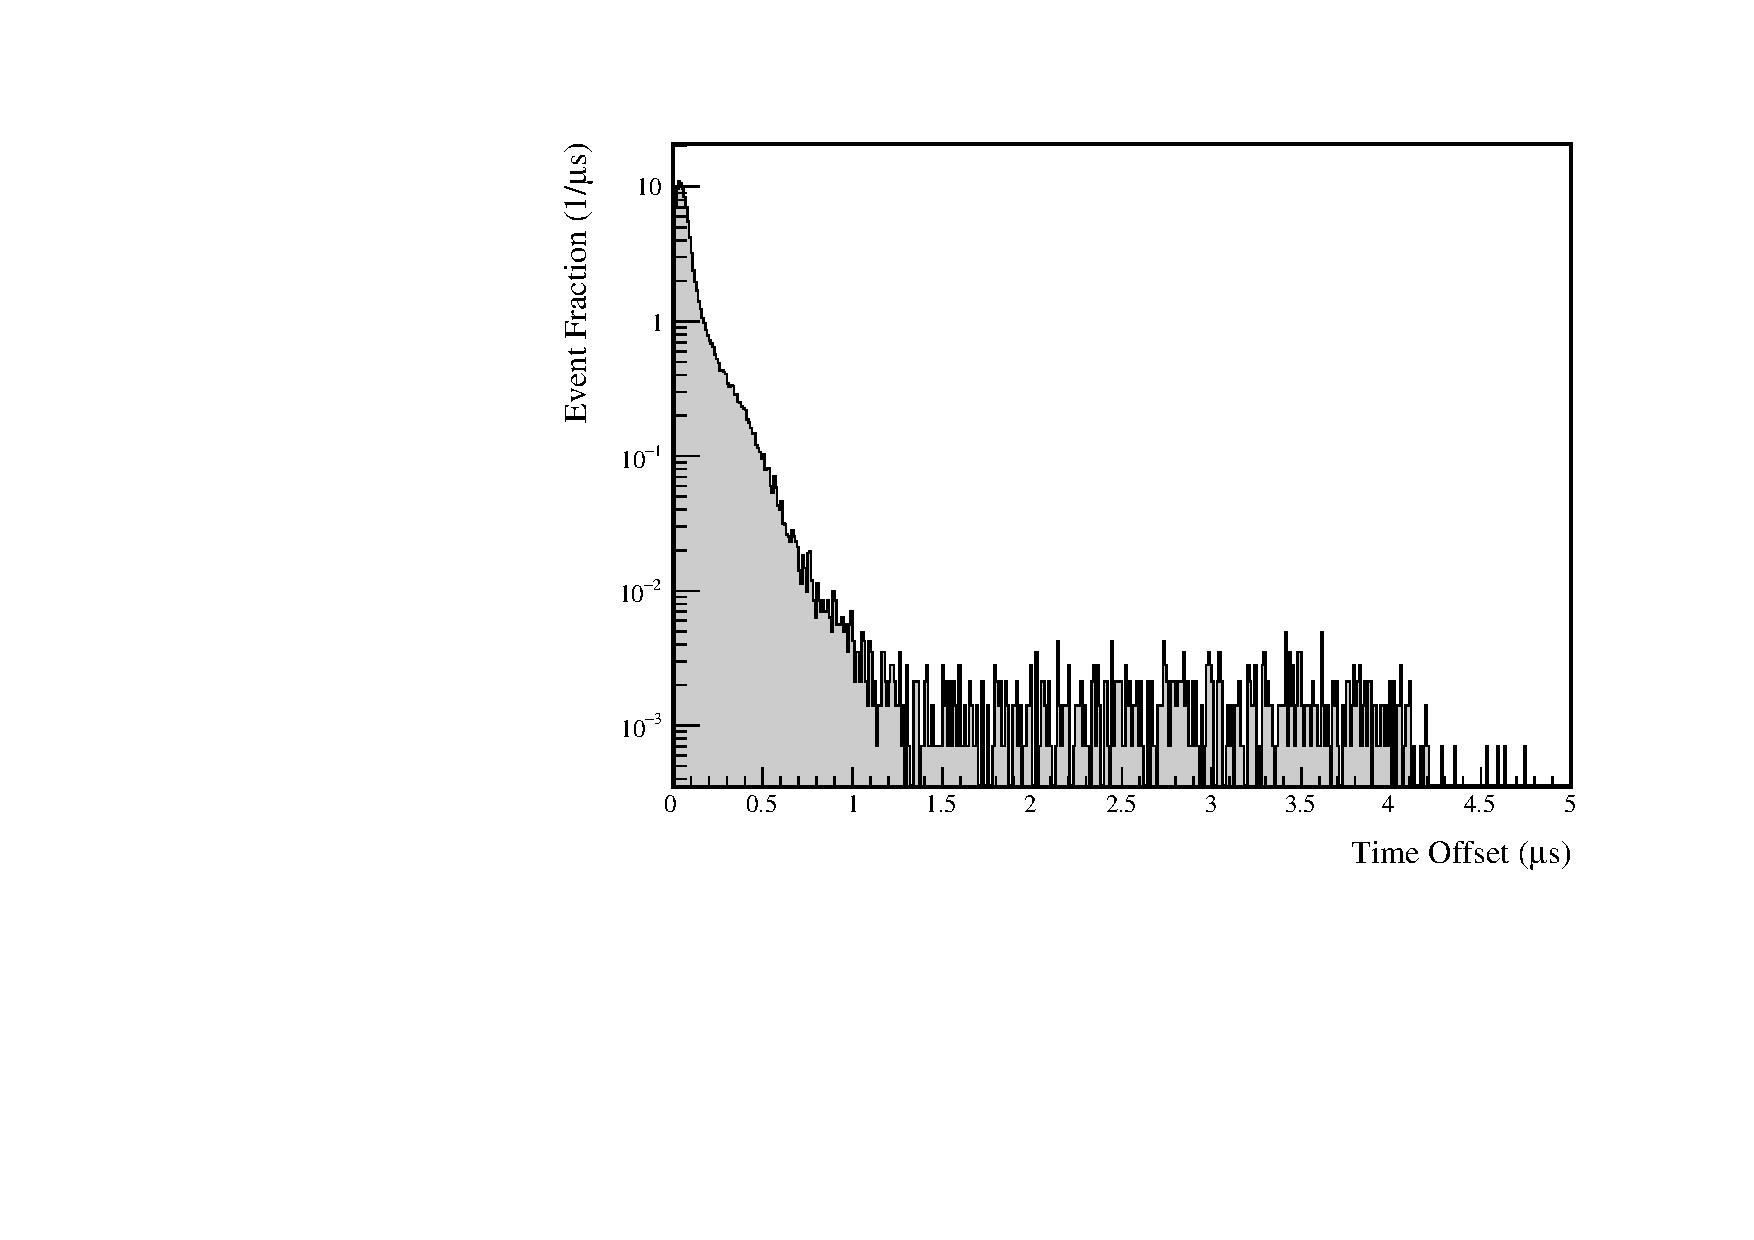
\includegraphics[width=0.8\textwidth]{toffset}
  \caption[Distribution of offset times within multi-detector events]{\label{fig:toffset}
    Distribution of time interval between individual hits within a multi-detector event during a \Th{228} calibration run. Offsets of greater than $\sim1.5$~$\mu$s are due to pileup, which is significant due to the high data rate of calibration runs.}
\end{figure}

\subsection{Variation in Detector Configuration} \label{sec:sds}
Throughout the runtime of the \MJD, not all detectors were simultaneously active, and within each dataset, the set of active detectors varied signficantly.
Because we are looking at \msmd\ events, the detection efficiency for \bbes\ events in any detector depends on which other detectors are enabled.
For this reason, detection efficiency is computed for each module in its entirety rather than for individual detectors.
To account for changes in detector configuration, each dataset is divided into subdatasets based on which detectors are active.
The subdatasets are described by a pair of 64-bit masks, one for each module, with each bit representing a single detector's state.
To decode the bitmask, the $b$'th least significant bit represents string position $P$, detector position $D$ if
\begin{equation}\label{eq:sdsbitmask}
  b = 8\cdot P + D
\end{equation}
The set of runs and active channels for each run were determined by the run selection and data cleaning committee, and the procedures are outlined in \cite{2018Reine}.
The program \texttt{es\_getdatasets} uses these selections to sort each run into a subdataset.
\\
The detection efficiency is defined as the probability of a signal event in any detector, including inactive detectors.
Detection efficiencyis calculated individually for each subdataset and for each module by creating separate a separate skim file for each subdataset as outlined in section~\ref{sec:simskim}.
The final efficiency is then computed as a isotopic exposure weighted average of the efficiency within each subdataset.
Any efficiency uncertainties are assumed to be totally correlated between subdatasets, meaning they are added linearly instead of in quadrature.
The livetime of each subdataset is calculated by the program \texttt{es\_livetimes} by totalling the run time in each run, and subtracting any deadtime that affects the entire module, including deadtime caused by the muon veto system and by liquid nitrogen fills.
Additional sources of deadtime that affect individual detectors are calculated as inefficiencies rather than being subtracted from the livetime, as discussed in section~\ref{sec:simskim}
This is done because deadtime in any individual detector affects the detection efficiency of all other detectors.
The isotopic exposure is computed by multiplying the livetime of each module of the total isotopic mass in each module, including mass in inactive detectors and dead layers.
Table~\ref{tab:subdatasets} lists each subdataset along with its livetime and exposure.

\scriptsize
\begin{longtabu}{|c|c c|c|c c|c c|c|}
  \hline
  DS & M1 Detector Mask & M2 Detector Mask & \makecell{Run Time\\(days)} & \makecell{M1 L.T.\\(days)} & M1 Eff. & \makecell{M2 L.T.\\(days)} & M2 Eff. & \makecell{Exposure\\(kg$\cdot$y)} \\
  \hline
\endfirsthead
  \hline
  DS & M1 Detector Mask & M2 Detector Mask & \makecell{Run Time\\(days)} & \makecell{M1 L.T.\\(days)} & M1 Eff. & \makecell{M2 L.T.\\(days)} & M2 Eff. & \makecell{Exposure\\(kg$\cdot$y)} \\
  \hline
\endhead
  \hline
  \multicolumn{9}{r}{\textit{Continued on the next page}} \\
  \caption{List of subdatasets}
\endfoot
  \hline
  \caption[List of subdatasets, livetimes, efficiency and exposure]{\label{tab:subdatasets}
    List of each subdataset with its livetime, detection efficiency measured for the \bbes to \SP{0}{+}{1} decay, and total isotopic exposure. Note the large amount of variance in the detection efficiency.
  }
\endlastfoot
  DS1 & 061a08001e0e1c00 & 0000000000000000 & 2.64 & 2.60 & 1.693\% & 0.00 & 0.000\% & 0.109 \\
  DS1 & 161a08341e0e1c00 & 0000000000000000 & 0.02 & 0.02 & 1.978\% & 0.00 & 0.000\% & 0.001 \\
  DS1 & 161a0c341e0e1c00 & 0000000000000000 & 4.51 & 4.48 & 1.915\% & 0.00 & 0.000\% & 0.188 \\
  DS1 & 161a0c361e0e1c00 & 0000000000000000 & 3.49 & 3.48 & 1.449\% & 0.00 & 0.000\% & 0.146 \\
  DS1 & 1e1a00001e0e1c00 & 0000000000000000 & 7.82 & 7.73 & 2.015\% & 0.00 & 0.000\% & 0.324 \\
  DS1 & 1e1a08001e0e1c00 & 0000000000000000 & 25.49 & 25.19 & 2.202\% & 0.00 & 0.000\% & 1.057 \\
  DS1 & 1e1a08041e0e1c00 & 0000000000000000 & 2.95 & 2.93 & 2.277\% & 0.00 & 0.000\% & 0.123 \\
  DS1 & 1e1a08141e0e1c00 & 0000000000000000 & 0.26 & 0.25 & 2.297\% & 0.00 & 0.000\% & 0.011 \\
  DS1 & 1e1a08301e0e1c00 & 0000000000000000 & 1.40 & 1.37 & 2.305\% & 0.00 & 0.000\% & 0.057 \\
  DS1 & 1e1a08341e0e1c00 & 0000000000000000 & 7.58 & 7.50 & 2.095\% & 0.00 & 0.000\% & 0.315 \\
  DS1 & 1e1a0c001e0e1c00 & 0000000000000000 & 1.96 & 1.93 & 2.226\% & 0.00 & 0.000\% & 0.081 \\
  DS1 & 1e1a0c341e0e1c00 & 0000000000000000 & 0.67 & 0.67 & 2.296\% & 0.00 & 0.000\% & 0.028 \\
  DS2 & 1e1a08001e0e1c00 & 0000000000000000 & 9.58 & 9.51 & 2.248\% & 0.00 & 0.000\% & 0.399 \\
  DS3 & 1e1a0c3e1e0e1c00 & 0000000000000000 & 29.88 & 29.67 & 2.566\% & 0.00 & 0.000\% & 1.245 \\
  DS4 & 0000000000000000 & 1c061a16060e1e00 & 19.15 & 0.00 & 0.000\% & 18.85 & 1.811\% & 0.622 \\
  DS5a & 08000020040e1c00 & 18060a02040e1e00 & 1.49 & 1.48 & 0.703\% & 1.46 & 1.111\% & 0.110 \\
  DS5a & 08080020040e1c00 & 18060a16060e1e00 & 2.51 & 2.49 & 0.842\% & 2.47 & 1.484\% & 0.186 \\
  DS5a & 08080030040e1c00 & 18060a02040e1e00 & 0.01 & 0.01 & 0.888\% & 0.01 & 1.094\% & 0.001 \\
  DS5a & 0e1a04321e0e1c00 & 08020a16060e1e00 & 2.69 & 2.71 & 2.265\% & 2.66 & 1.165\% & 0.201 \\
  DS5a & 0e1a0c321e0e1c00 & 0000000000000000 & 0.65 & 0.63 & 2.522\% & 0.00 & 0.000\% & 0.026 \\
  DS5a & 0e1a0c321e0e1c00 & 08060a16060e1e00 & 1.24 & 1.24 & 2.513\% & 1.21 & 1.451\% & 0.092 \\
  DS5a & 0e1a0c321e0e1c00 & 18060a02040e1e00 & 2.94 & 2.92 & 2.288\% & 2.89 & 1.098\% & 0.218 \\
  DS5a & 0e1a0c321e0e1c00 & 18060a1406061600 & 0.04 & 0.04 & 2.487\% & 0.04 & 0.906\% & 0.003 \\
  DS5a & 0e1a0c321e0e1c00 & 18060a1606060600 & 3.19 & 3.15 & 2.452\% & 3.16 & 0.774\% & 0.237 \\
  DS5a & 0e1a0c321e0e1c00 & 18060a16060e0600 & 3.30 & 3.28 & 2.458\% & 3.29 & 0.793\% & 0.246 \\
  DS5a & 0e1a0c3e1e0e1c00 & 1806020606081800 & 1.75 & 1.73 & 2.703\% & 1.73 & 0.726\% & 0.129 \\
  DS5a & 0e1a0c3e1e0e1c00 & 18060216060c1c00 & 6.84 & 6.77 & 2.698\% & 6.74 & 1.068\% & 0.507 \\
  DS5a & 0e1a0c3e1e0e1c00 & 18060216060e1e00 & 13.48 & 13.30 & 2.677\% & 13.27 & 1.189\% & 0.996 \\
  DS5a & 0e1a0c3e1e0e1c00 & 18060816060e1c00 & 0.05 & 0.05 & 2.502\% & 0.05 & 1.247\% & 0.004 \\
  DS5a & 0e1a0c3e1e0e1c00 & 18060a0606060c00 & 2.16 & 2.12 & 2.670\% & 2.12 & 0.982\% & 0.159 \\
  DS5a & 0e1a0c3e1e0e1c00 & 18060a16040e1e00 & 0.76 & 0.76 & 2.668\% & 0.74 & 1.222\% & 0.056 \\
  DS5a & 0e1a0c3e1e0e1c00 & 18060a1606060c00 & 0.25 & 0.25 & 2.682\% & 0.25 & 1.060\% & 0.019 \\
  DS5a & 0e1a0c3e1e0e1c00 & 18060a1606061800 & 1.88 & 1.86 & 2.686\% & 1.86 & 0.998\% & 0.140 \\
  DS5a & 0e1a0c3e1e0e1c00 & 18060a1606061c00 & 9.20 & 9.13 & 2.657\% & 9.06 & 1.353\% & 0.682 \\
  DS5a & 0e1a0c3e1e0e1c00 & 18060a16060c1c00 & 7.89 & 7.79 & 2.688\% & 7.79 & 1.350\% & 0.584 \\
  DS5a & 0e1a0c3e1e0e1c00 & 18060a16060e1c00 & 11.68 & 11.53 & 2.340\% & 11.51 & 1.357\% & 0.864 \\
  DS5a & 0e1a0c3e1e0e1c00 & 18060a16060e1e00 & 5.21 & 5.15 & 2.665\% & 5.13 & 1.486\% & 0.386 \\
  DS5a & 0e1a0c3e1e0e1c00 & 18061216060e1e00 & 2.39 & 2.37 & 2.676\% & 2.37 & 1.266\% & 0.178 \\
  DS5b & 1e1a0c3e1e0c1c00 & 18061216060e1e00 & 24.46 & 24.09 & 2.672\% & 24.06 & 1.268\% & 1.805 \\
  DS5b & 1e1a0c3e1e0c1c00 & 18061a16060e1e00 & 0.75 & 0.75 & 2.670\% & 0.75 & 1.654\% & 0.056 \\
  DS5b & 1e1a0c3e1e0e1c00 & 18061216060e1e00 & 14.28 & 14.12 & 2.766\% & 14.07 & 1.169\% & 1.057 \\
  DS5c & 1e1a0c3e1e0c1c00 & 00060216060e0e00 & 0.00 & 0.00 & 2.567\% & 0.00 & 0.787\% & 0.000 \\
  DS5c & 1e1a0c3e1e0c1c00 & 00060a16060e0e00 & 0.91 & 0.89 & 2.664\% & 0.91 & 1.016\% & 0.067 \\
  DS5c & 1e1a0c3e1e0c1c00 & 00061216060e0e00 & 10.22 & 10.15 & 2.645\% & 10.03 & 0.857\% & 0.757 \\
  DS6a & 12000000000c0800 & 1002020006040600 & 1.33 & 1.31 & 0.160\% & 1.31 & 0.230\% & 0.099 \\
  DS6a & 12000c20000c1c00 & 18061216060c1600 & 6.93 & 6.84 & 0.756\% & 6.86 & 0.679\% & 0.514 \\
  DS6a & 12020000040c0800 & 1802020006040600 & 1.30 & 1.28 & 0.284\% & 1.28 & 0.275\% & 0.096 \\
  DS6a & 12020c00040c1800 & 1802020006040600 & 2.37 & 2.33 & 0.676\% & 2.33 & 0.275\% & 0.175 \\
  DS6a & 12080c20000c1c00 & 18061216060c1600 & 3.38 & 3.34 & 0.931\% & 3.34 & 0.677\% & 0.251 \\
  DS6a & 12120c3e1c0c1c00 & 18061216060c1600 & 0.56 & 0.54 & 1.847\% & 0.56 & 0.676\% & 0.041 \\
  DS6a & 16020c10040c1800 & 1806020006060600 & 3.23 & 3.20 & 0.883\% & 3.19 & 0.416\% & 0.239 \\
  DS6a & 160a0c321c0c1c00 & 1806021006061600 & 1.98 & 1.95 & 2.022\% & 1.97 & 0.521\% & 0.147 \\
  DS6a & 1e0a0c321c0c1c00 & 1806020006040200 & 2.62 & 2.59 & 2.275\% & 2.59 & 0.260\% & 0.194 \\
  DS6a & 1e0a0c321c0c1c00 & 1806020006040600 & 1.31 & 1.29 & 2.275\% & 1.29 & 0.390\% & 0.097 \\
  DS6a & 1e0a0c321c0c1c00 & 1806020006041600 & 1.30 & 1.28 & 2.275\% & 1.26 & 0.459\% & 0.096 \\
  DS6a & 1e0a0c321c0c1c00 & 1806021006061600 & 1.61 & 1.59 & 2.275\% & 1.59 & 0.521\% & 0.119 \\
  DS6a & 1e120c3e1c0c1c00 & 18061216060c1600 & 0.95 & 0.93 & 2.284\% & 0.93 & 0.676\% & 0.070 \\
  DS6a & 1e1a0c321c0c1c00 & 1806020006060600 & 1.30 & 1.28 & 2.457\% & 1.28 & 0.416\% & 0.096 \\
  DS6a & 1e1a0c321c0c1c00 & 1806021006040600 & 3.91 & 3.88 & 2.457\% & 3.87 & 0.415\% & 0.291 \\
  DS6a & 1e1a0c321c0c1c00 & 1806021006041600 & 2.92 & 2.90 & 2.457\% & 2.90 & 0.495\% & 0.217 \\
  DS6a & 1e1a0c321c0c1c00 & 1806021006060600 & 1.31 & 1.30 & 2.455\% & 1.30 & 0.436\% & 0.097 \\
  DS6a & 1e1a0c3a1c0c1c00 & 1806020006040600 & 2.32 & 2.31 & 2.553\% & 2.32 & 0.390\% & 0.174 \\
  DS6a & 1e1a0c3a1c0c1c00 & 1806021006040600 & 1.77 & 1.77 & 2.552\% & 1.75 & 0.415\% & 0.132 \\
  DS6a & 1e1a0c3a1c0c1c00 & 1806021006041600 & 0.67 & 0.67 & 2.553\% & 0.67 & 0.494\% & 0.050 \\
  DS6a & 1e1a0c3e1c0c1c00 & 1806000006040600 & 2.22 & 2.18 & 2.631\% & 2.16 & 0.360\% & 0.163 \\
  DS6a & 1e1a0c3e1c0c1c00 & 1806020006041600 & 1.32 & 1.30 & 2.630\% & 1.30 & 0.458\% & 0.097 \\
  DS6a & 1e1a0c3e1c0c1c00 & 1806021006041600 & 1.30 & 1.28 & 2.630\% & 1.28 & 0.494\% & 0.096 \\
  DS6a & 1e1a0c3e1c0c1c00 & 18060210060c1600 & 4.63 & 4.58 & 2.629\% & 4.55 & 0.533\% & 0.342 \\
  DS6a & 1e1a0c3e1c0c1c00 & 1806021206041600 & 2.61 & 2.56 & 2.628\% & 2.57 & 0.515\% & 0.192 \\
  DS6a & 1e1a0c3e1c0c1c00 & 18060214060c0600 & 1.70 & 1.70 & 2.628\% & 1.68 & 0.492\% & 0.127 \\
  DS6a & 1e1a0c3e1c0c1c00 & 18060214060c1600 & 1.38 & 1.36 & 2.627\% & 1.36 & 0.576\% & 0.102 \\
  DS6a & 1e1a0c3e1c0c1c00 & 18060214060e1600 & 23.42 & 23.19 & 2.601\% & 23.12 & 0.555\% & 1.736 \\
  DS6a & 1e1a0c3e1c0c1c00 & 18061212060c1600 & 2.93 & 2.89 & 2.628\% & 2.90 & 0.644\% & 0.217 \\
  DS6a & 1e1a0c3e1c0c1c00 & 18061216060c1600 & 6.59 & 6.51 & 2.628\% & 6.51 & 0.690\% & 0.488 \\
  \hline
  DSTotal & -- & -- & 321.60 & 318.26 & 2.354\% & 238.53 & 0.987\% & 21.228 \\

\end{longtabu}
\normalsize

\subsection{Dead Layer Effects} \label{sec:DL}
For \msmd\ events, each individual hit may be degraded by the deadlayer, so the loss of sensitivity from deadlayers is larger for this search than for searches for single-site events.
For this reason, dead layer effects are treated as a loss of detection efficiency instead of a loss of exposure.
Dead layers are included in the simulations as a part of post-processing as described in section~\ref{sec:simpostproc}
To account for uncertainty in the thickness of the deadlayer, two separate simulations are run, with and without deadlayers.
By comparing the efficiency measurement from each simulation, we measure the size of the dead layer effect.
The percent uncertainty in the efficiency loss from dead layers is assumed to be the same as the percent uncertainty in the dead layer thickness.
Typical loss of efficiency for multi-site peaks is 25-35\%; for the \tnbb\ to the \SP{0}{+}{1} decay, the losses are 26\% for module~1 and 34\% for module~2.
The uncertainty in the dead layer tends to be one of the dominant uncertainties in measuring the detection efficiency.
The effect of dead layers on detection efficiency can be seen in figure~\ref{fig:dldt}.
\\
\begin{figure}
  \centering
  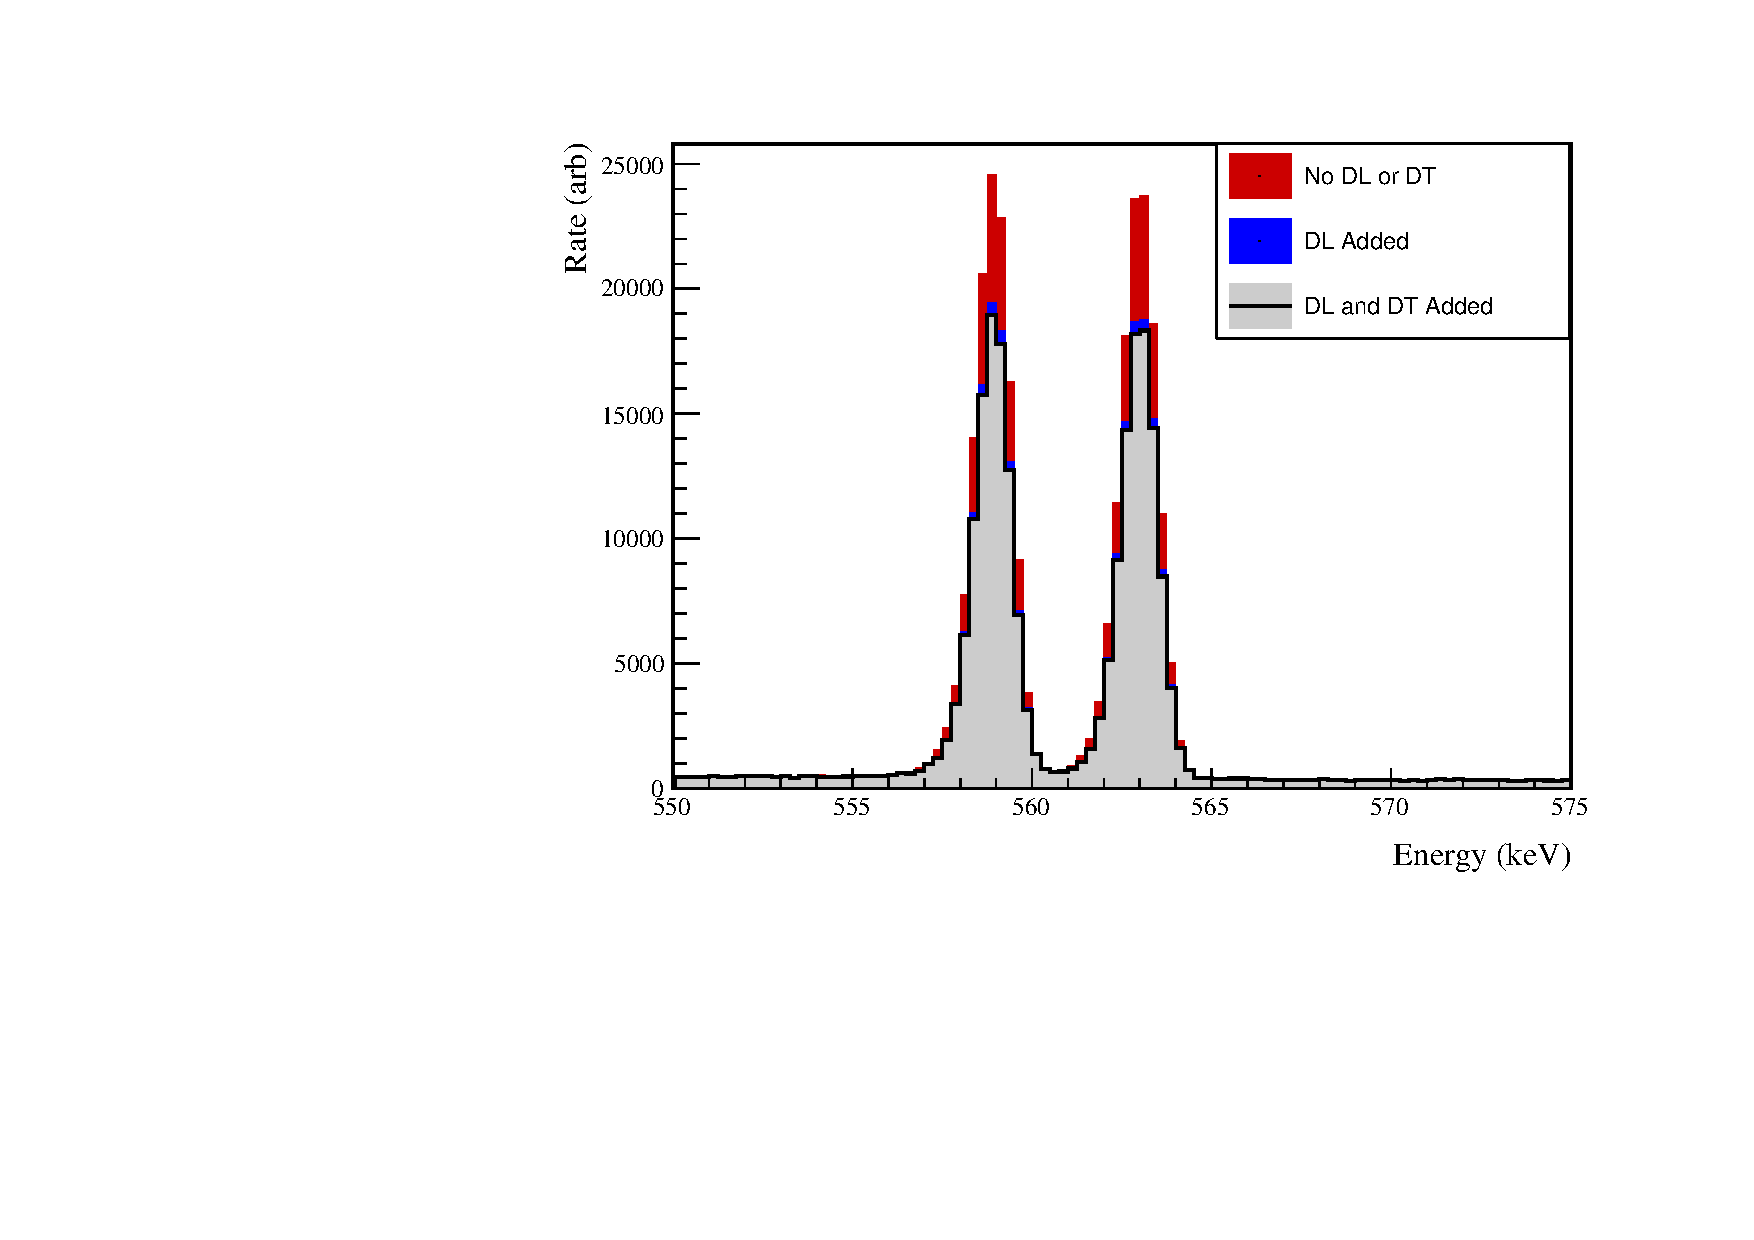
\includegraphics[width=0.8\textwidth]{DeadLayerDeadTime}
  \caption[Simulated effect of dead layers and dead times]{\label{fig:dldt}
    Effect of dead layers and dead times on peak amplitudes for \tnbb\ to the \SP{0}{+}{1} peaks in \msmd\ events.
  }
\end{figure}

\subsection{Dead Time Effects} \label{sec:DT}
Detector deadtimes, which affect only a single detector simultaneously, reduce the detection efficiency for events that occur in all detectors in the module.
For this reason, instead of subtracting these deadtimes from the livetime, the deadtimes are incorperated into the detection efficiency.
Detector deadtimes are measured individually for each run by counting pulser events and comparing to the number of expected pulser events for each detector.
\texttt{es\_livetime} collects the detector deadtimes that are measured in this way and finds the average detector deadtime for each subdataset.
These dead times are then applied to the simulation skimming process as described in section~\ref{sec:simskim}.
Similar to the dead layers, simulation files are produced with and without deadtimes in order to measure the size of the effect.
Uncertainties in the detector deadtimes are measured as the statistical uncertainties from pulser counts.
The percent uncertainty in efficiency loss from detector dead times is assumed to be the same as the average percent uncertainty in the detector dead time.
Typical loss of efficiency from detector deadtims range from 1-3\%.
For the \tnbb\ to the \SP{0}{+}{1} decay, the losses are 2.5\% for module~1 and 1.9\% for module~2.
The effects of detector deadtimes can be seen in figure~\ref{fig:dldt}.
\\
\subsection{Additional Effects} \label{sec:Co56}
Other possible sources of systematic uncertainty, which could hypothetically result from inaccuracies in the simulation geometry, in the detection efficiency must be accounted for.
To do so, we use pair production events from calibration runs as a proxy for \bbes\ events.
In pair production events, an electron-positron pair is produced in the bulk of a detector, followed promptly by two 511~keV $\gamma$s from the annihilation of the positron.
Because these events involve a single pair production site and the prompt emission of gamma rays which may be absorbed in a separate detector, they make a good proxy for \bbes\ events.
In single-escape peak (SEP) events, one gamma is absorbed in the same detector as the pair-production, while the other escapes, resulting in a detector hit with energy equal to the $\gamma$ energy minus 511~keV.
In double-escape peak (DEP) events, both gammas escape the detector, resulting in a detector hit with energy equal to the $\gamma$ energy minus 1022~keV.
Both both SEP and DEP events present the possibility for a second 511~keV detector hit.
By comparing the rate of multiplicity-1 events in the SEPs and DEPs to the rate of multiplicity-2 events in which one hit falls into one of these peaks and the other falls into the 511~keV peak, we can measure a proxy the detection efficiency of our multi-site event signature.
By comparing this measurement to simulation, we can estimate the size of any unknown uncertainties in our simulation-based efficiency estimate.
\\
\begin{figure}[ht]
  \centering
  \subfloat{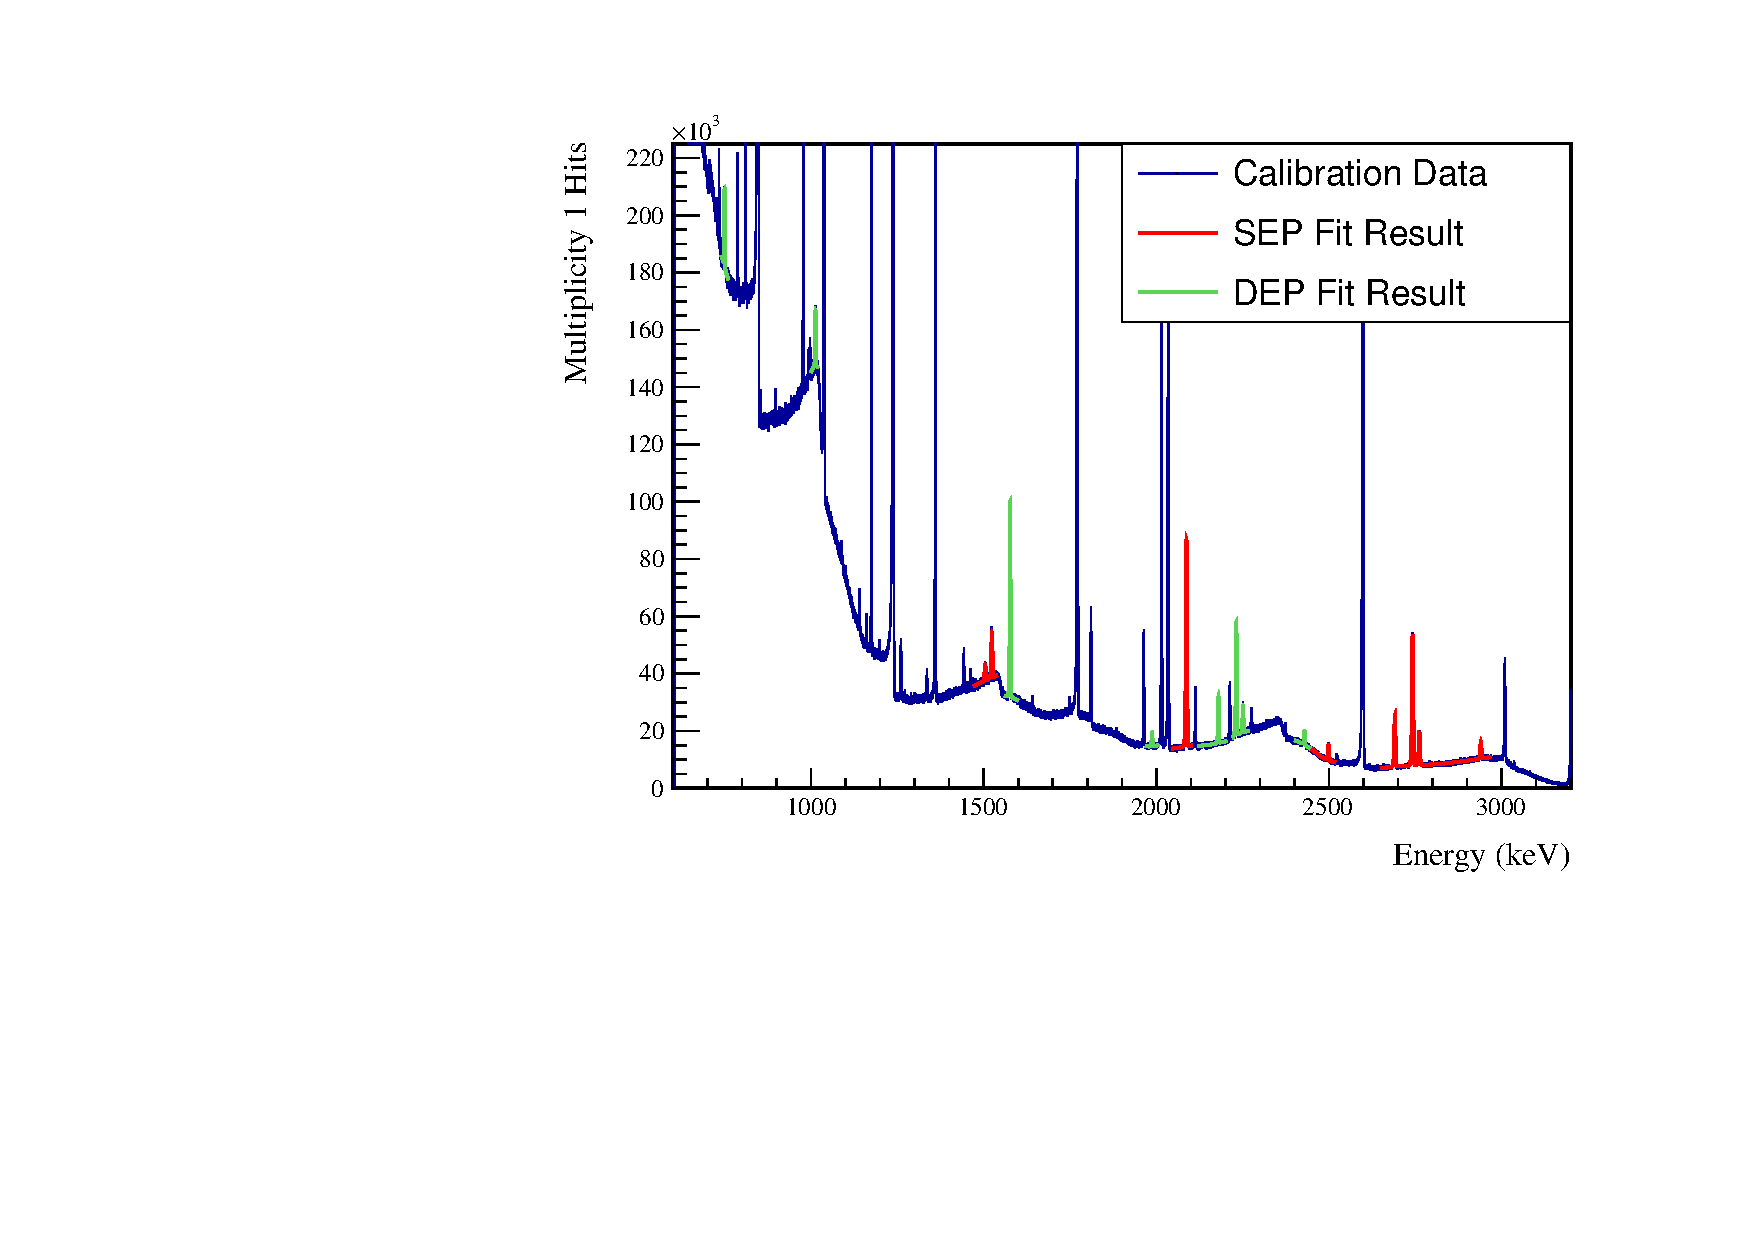
\includegraphics[width=.5\linewidth]{mult1Co56Fits}}
  \subfloat{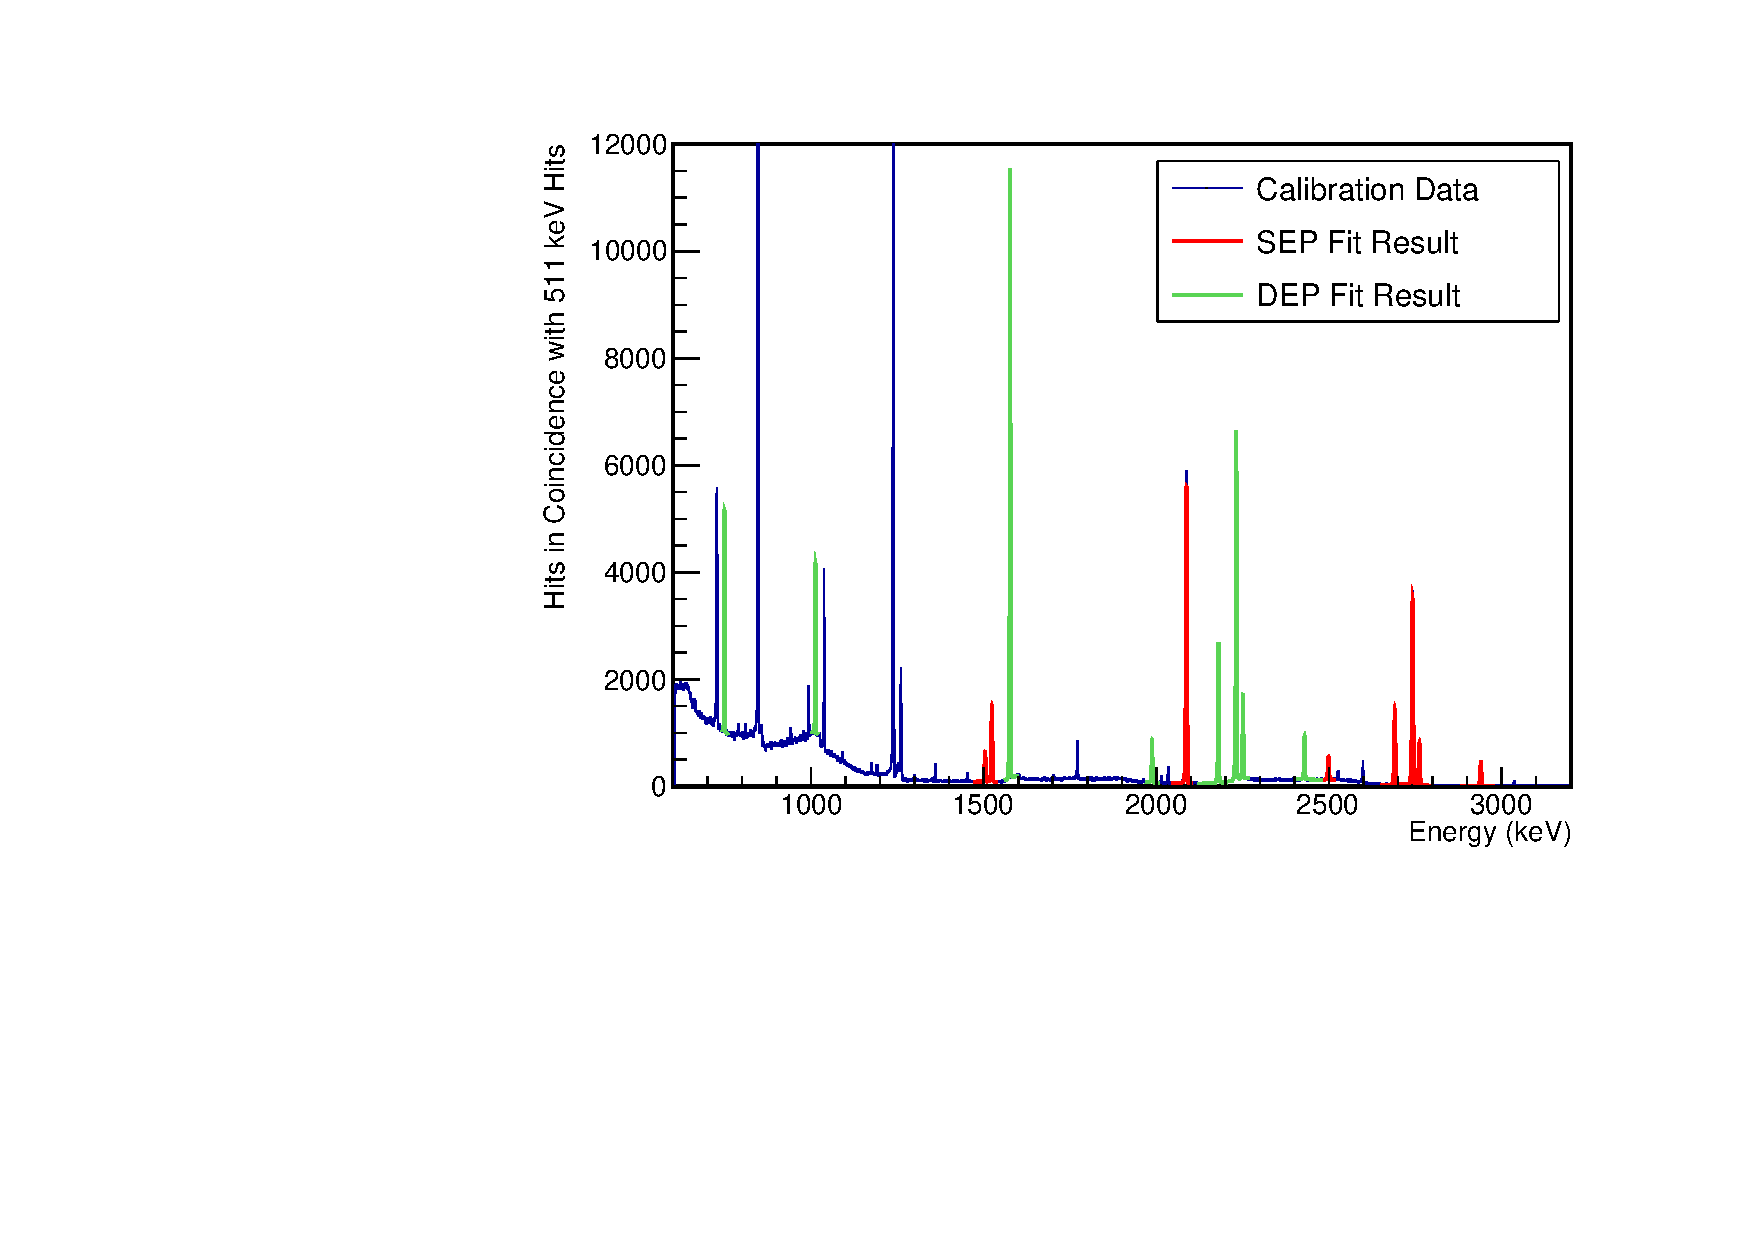
\includegraphics[width=.5\linewidth]{mult2Co56Fits}}
  \caption[Spectra of multiplicty 1 and 2 \Co{56} data with peak fits]{\label{fig:Co56Spectra}
    Spectra of multiplicity 1 \Co{56} events (left) and multiplicity 2 \Co{56} events in coincidence with an annihilation gamma. The results of the simultaneous peak fits are drawn in red (SEP fit) and green (DEP fit).
  }
\end{figure}
To achieve this, we will use a \Co{56} calibration source.
\Co{56} presents the advantage of a large number of $\gamma$s at energies high enough to cause pair production, which allows for a comparison of many peaks to our simulation.
A \Co{56} line source was inserted into the module~1 calibration track on January 15, 2019 and was 168.1~hrs of data were recorded, until January 22, 2019.
Immediately after this, the source was inserted into the module~2 calibration track and 167.1~hrs of data were recorded until January 29, 2019.
The source had a nominal activity of 6~kHz, resulting in a high enough data rate that the energy threshold for each channel was raised to $\sim400$~keV.
As discussed in section~\ref{sec:calsims}, 3~billion event primaries were simulated for the \Co{56} source in each module's source track in order to achieve similar events statistics for both the simulations and data.
Simulations were run with and without dead-layers.
\\
8 SEPs and 7 DEPs were selected as proxies for the \bbes\ signal.
A simultaneous fit, as described in appendix~\ref{app:peakshape}, of all SEPs as single-detector events and as two-detector events in coincidence with a 511~keV peak event was performed in the calibration data and in the simulations both with and without dead layers.
SEPs and DEPs have abnormal peakshapes due to in flight annihilation of the positrons, which results in Doppler broadening of the peak shapes.
For this reason, a high energy tail is added to the typical peak shape function.
The peak height ratios and uncertainties for peak $k$ are determined as follows:
\begin{equation}
  \epsilon_k=\frac{A_{k,m2}}{A_{k,m1}}
\end{equation}
\begin{equation}
  \sigma_{stat, k}=\epsilon_k \sqrt{\frac{\Sigma_{A,k,m1;A,k,m1}}{A_{k,m1}^2}-2\frac{\Sigma_{A,k,m1;A,k,m2}}{A_{k,m1}A_{k,m2}}+\Sigma_{A,k,m2;A,k,m2}}{A_{k,m2}^2}
\end{equation}
where $A_{k,m1/2}$ are the fitted amplitudes of peak $k$ with multiplicity 1 and multiplicity 2 respectively, and $\Sigma_{A,k,m1/2;A,k,m1/2}$ is the fitter covariance matrix element for these amplitudes.
The same process of simultaneously fitting DEPs is followed to extract the DEP peak-height ratios.
The measured data spectra and fit results are shown in figure~\ref{fig:Co56Spectra}.
\\
\begin{figure}[p]
  \centering
  \subfloat[Module 1]{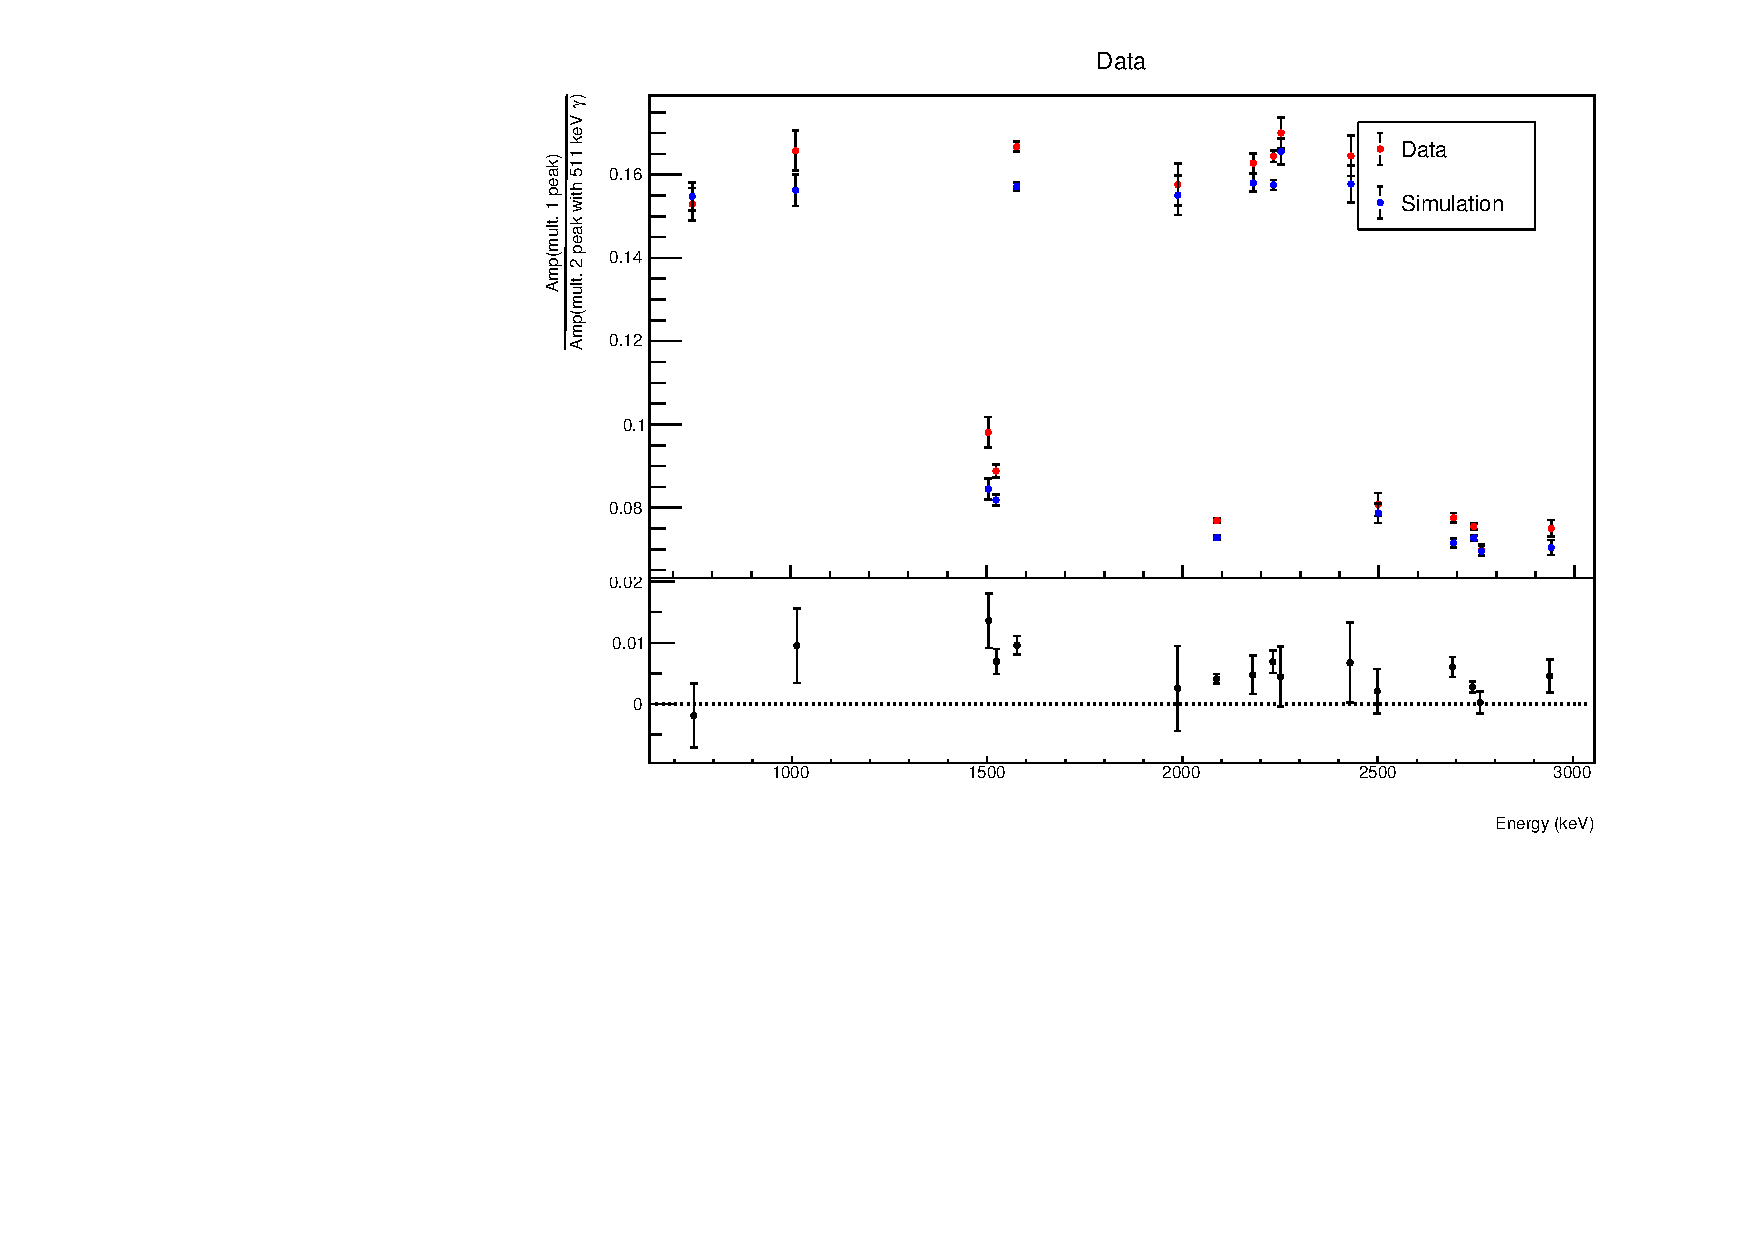
\includegraphics[width=.75\linewidth]{M1PeakRatioComparison}}
  \\
  \subfloat[Module 2]{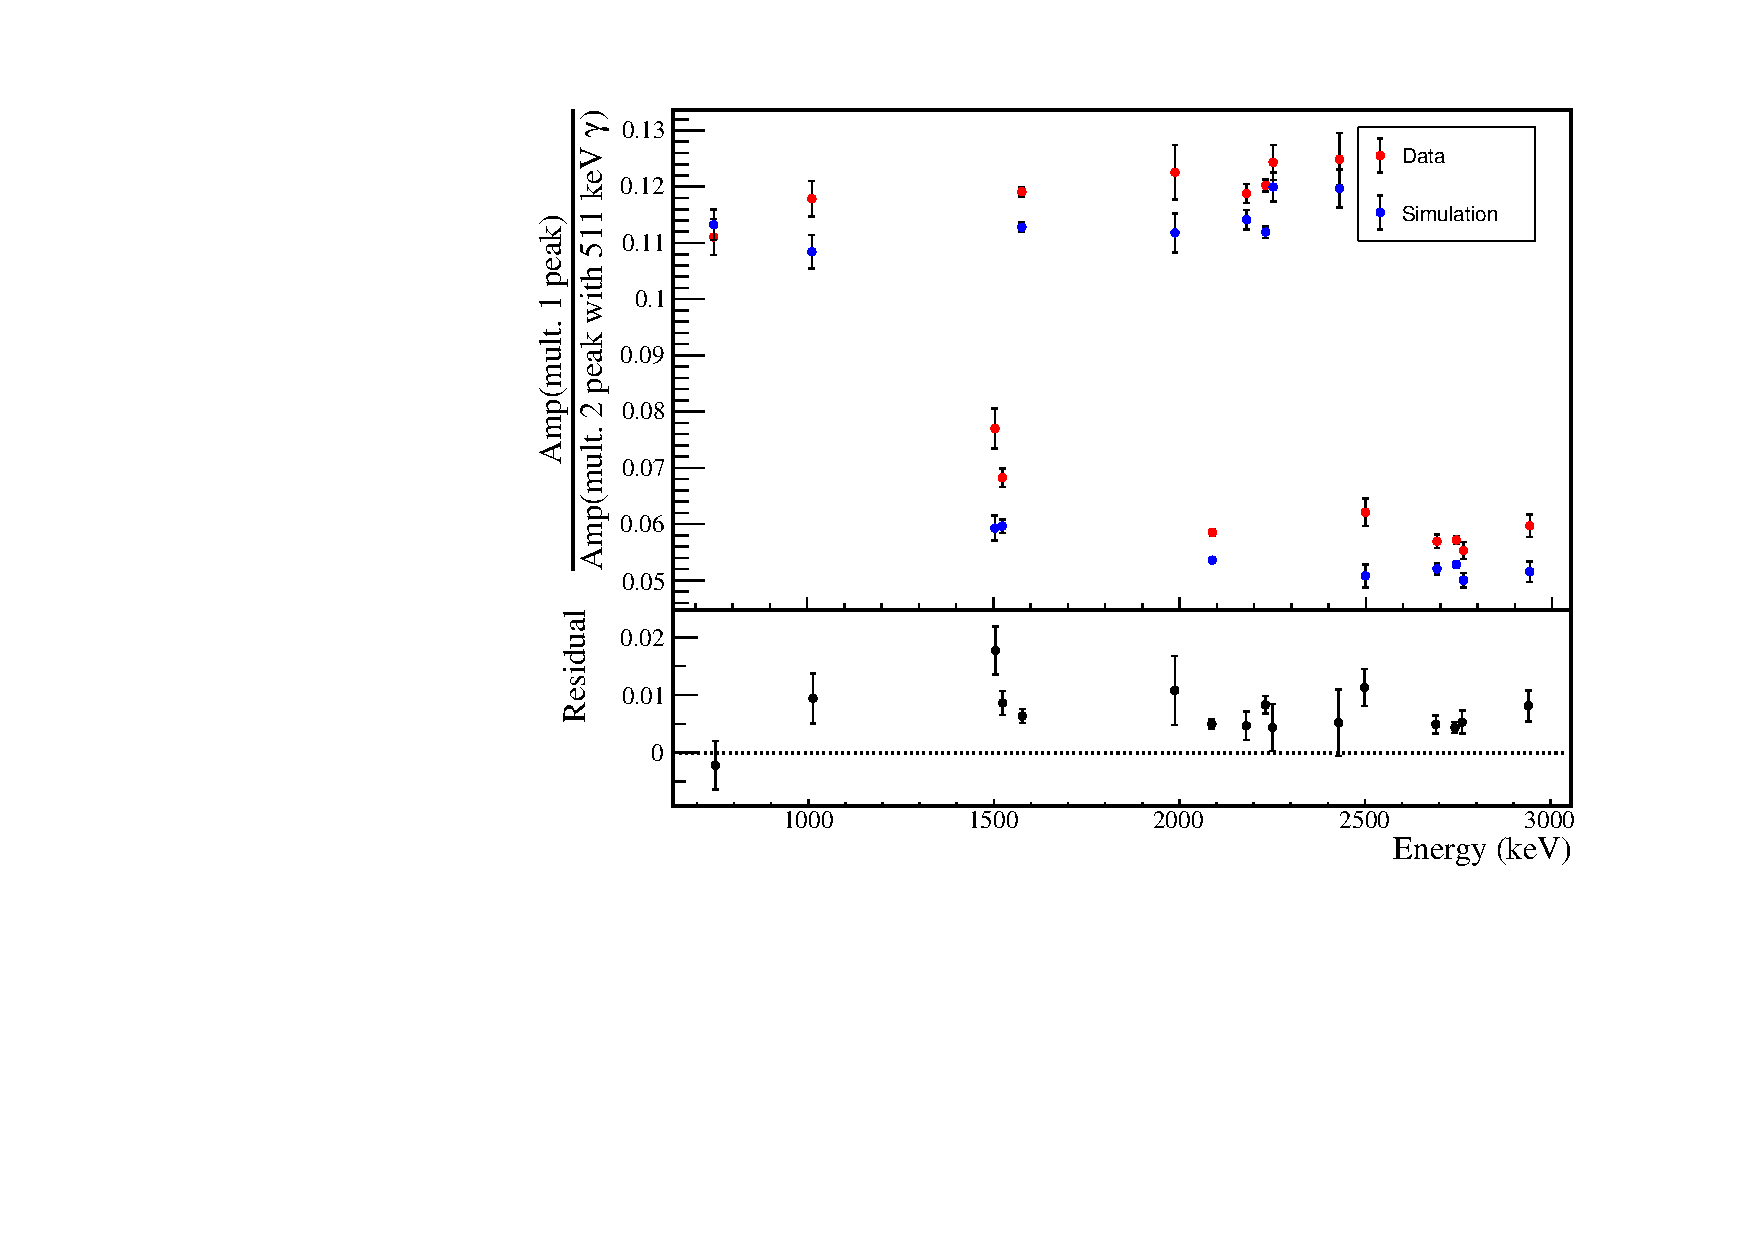
\includegraphics[width=.75\linewidth]{M2PeakRatioComparison}}
  \caption[Peak height ratio comparison results for module 1 and module 2]{\label{fig:co56results}
    Measurement of peak height ratios between multiplicity~1 events and multiplicity~2 events containing a 511~keV annihalation $\gamma$ for both simulated and measured \Co{56} spectra. Only statistical error bars are drawin. These ratios are listed in tables~\ref{tab:co56resultsM1} and \ref{tab:co56resultsM2}.
  }
\end{figure}
Any discrepancy between the simulated and measured data is treated as a systematic error which will be applied to the \bbes\ measurement.
Since some of this discrepancy can be explained by the dead layer uncertainty, the difference between the simulated peak-height ratios with and without the deal layer is multiplied by the percent uncertainty in the dead layer thickness in order to measure the systematic error caused by the dead layer.
Finally, a $\chi^2$ value is computed for the comparison between the simulated and measured peak-heights using the statistical and dead-layer uncertainties.
\begin{equation}
  \chi^2 = \displaystyle\sum_{k=1}^N \frac{(\epsilon_{k, meas}-\epsilon_{k, sim}-\delta_{DL}\cdot\sigma_{DL,k} - \mu)^2}{\sigma_{stat,dat,k}^2+\sigma_{stat,sim,k}^2} + \delta_{DL}^2
\end{equation}
where $\delta_{DL}$ is the error from the deal layer thickness, which is correlated across all peaks, and $\mu$ is the mean error that remains.
This $\chi^2$ function is minimized, and the systematic error is taken to be
\begin{equation}
  \sigma_{sim}^2 = \mu^2 + \sigma_\mu^2
\end{equation}
Tables~\ref{tab:co56resultsM1} and~\ref{tab:co56resultsM2} list the peak height ratios and uncertainties for each peak for module~1 and module~2, respectively.
The final fractional uncertainties measured are $\sigma_{sim,M1}=0.0020$ and $\sigma_{sim,M2}=0.0047$.
This uncertainty is applied directly to the detection efficiency measured before applying any other effects such as dead layers, dead times and cuts, without any scaling.
This uncertainty is one of the dominant uncertainties on the detection efficiency along with the dead layer uncertainty; while the absolute uncertainty is small, because it is applied to the detection efficiency, which tends to be $\sim5$\%, directly rather than to the loss from an individual effect, the fractional uncertaint is quite high.
In cases where the detection efficiency is very low, such as the 1216~keV peak in module~2 from decays to the \SP{2}{+}{2} state, this uncertainty can completely overwhelm the detection efficiency.
Figure~\ref{fig:co56results} plots the peak height ratios for simulated and measured data for both modules~1 and~2.

\begin{table}[p]
  \caption[Table of peak height ratios for module~1]{\label{tab:co56resultsM1}
    Table of measured peak height ratios between multiplicity~1 events and multiplicity~2 events containing a 511~keV annihalation $\gamma$ in module~1 for both simulated and measured \Co{56} spectra, with uncertainties. A plot of these numbers is shown in figure~\ref{fig:co56results}
  }
  \begin{tabular}{|c|c c c|c c c|c c|}
\hline
  Peak & $\frac{A_{m2,dat}}{A_{m1,dat}}$ & $\frac{A_{m2,sim}}{A_{m1,sim}}$ & $\frac{A_{m2,noDL}}{A_{m1,noDL}}$ & $\sigma_{dat,stat}$ & $\sigma_{sim,stat}$ & $\sigma_{sim,DL}$ & Residual & $\sigma_{resid}$ \\
\hline
  1504 keV (SEP) & 0.098 & 0.084 & 0.110 & 0.004 & 0.003 & 0.004 & 0.014 & 0.004 \\
  1524 keV (SEP) & 0.089 & 0.082 & 0.109 & 0.002 & 0.001 & 0.005 & 0.007 & 0.002 \\
  2088 keV (SEP) & 0.077 & 0.073 & 0.098 & 0.001 & 0.001 & 0.004 & 0.004 & 0.001 \\
  2499 keV (SEP) & 0.081 & 0.079 & 0.108 & 0.003 & 0.002 & 0.005 & 0.002 & 0.004 \\
  2691 keV (SEP) & 0.078 & 0.072 & 0.099 & 0.001 & 0.001 & 0.005 & 0.006 & 0.002 \\
  2743 keV (SEP) & 0.075 & 0.073 & 0.101 & 0.001 & 0.001 & 0.005 & 0.003 & 0.001 \\
  2762 keV (SEP) & 0.070 & 0.070 & 0.096 & 0.001 & 0.001 & 0.004 & 0.000 & 0.002 \\
  2940 keV (SEP) & 0.075 & 0.070 & 0.100 & 0.002 & 0.002 & 0.005 & 0.005 & 0.003 \\
  749 keV (DEP) & 0.153 & 0.155 & 0.225 & 0.004 & 0.003 & 0.012 & -0.002 & 0.005 \\
  1013 keV (DEP) & 0.166 & 0.156 & 0.229 & 0.005 & 0.004 & 0.012 & 0.010 & 0.006 \\
  1577 keV (DEP) & 0.167 & 0.157 & 0.224 & 0.001 & 0.001 & 0.011 & 0.010 & 0.002 \\
  1988 keV (DEP) & 0.158 & 0.155 & 0.222 & 0.005 & 0.005 & 0.011 & 0.003 & 0.007 \\
  2180 keV (DEP) & 0.163 & 0.158 & 0.225 & 0.002 & 0.002 & 0.011 & 0.005 & 0.003 \\
  2232 keV (DEP) & 0.164 & 0.158 & 0.225 & 0.001 & 0.001 & 0.012 & 0.007 & 0.002 \\
  2251 keV (DEP) & 0.170 & 0.166 & 0.233 & 0.004 & 0.003 & 0.011 & 0.004 & 0.005 \\
  2429 keV (DEP) & 0.165 & 0.158 & 0.230 & 0.005 & 0.004 & 0.012 & 0.007 & 0.007 \\
\hline
\end{tabular}

\end{table}

\begin{table}[p]
  \caption[Table of peak height ratios for module~2]{\label{tab:co56resultsM2}
    Table of measured peak height ratios between multiplicity~1 events and multiplicity~2 events containing a 511~keV annihalation $\gamma$ in module~2 for both simulated and measured \Co{56} spectra, with uncertainties. A plot of these numbers is shown in figure~\ref{fig:co56results}
  }
  \begin{tabular}{|c|c c c|c c c|c c|}
\hline
  Peak & $\frac{A_{m2,dat}}{A_{m1,dat}}$ & $\frac{A_{m2,sim}}{A_{m1,sim}}$ & $\frac{A_{m2,noDL}}{A_{m1,noDL}}$ & $\sigma_{dat,stat}$ & $\sigma_{sim,stat}$ & $\sigma_{sim,DL}$ & Residual & $\sigma_{resid}$ \\
\hline
  1504 keV (SEP) & 0.077 & 0.059 & 0.082 & 0.004 & 0.002 & 0.004 & 0.018 & 0.004 \\
  1524 keV (SEP) & 0.068 & 0.060 & 0.081 & 0.002 & 0.001 & 0.004 & 0.009 & 0.002 \\
  2088 keV (SEP) & 0.059 & 0.054 & 0.074 & 0.001 & 0.000 & 0.003 & 0.005 & 0.001 \\
  2499 keV (SEP) & 0.062 & 0.051 & 0.073 & 0.002 & 0.002 & 0.004 & 0.011 & 0.003 \\
  2691 keV (SEP) & 0.057 & 0.052 & 0.074 & 0.001 & 0.001 & 0.004 & 0.005 & 0.002 \\
  2743 keV (SEP) & 0.057 & 0.053 & 0.075 & 0.001 & 0.001 & 0.004 & 0.004 & 0.001 \\
  2762 keV (SEP) & 0.055 & 0.050 & 0.071 & 0.002 & 0.001 & 0.004 & 0.005 & 0.002 \\
  2940 keV (SEP) & 0.060 & 0.052 & 0.072 & 0.002 & 0.002 & 0.003 & 0.008 & 0.003 \\
  749 keV (DEP) & 0.111 & 0.113 & 0.155 & 0.003 & 0.003 & 0.007 & -0.002 & 0.004 \\
  1013 keV (DEP) & 0.118 & 0.108 & 0.156 & 0.003 & 0.003 & 0.008 & 0.009 & 0.004 \\
  1577 keV (DEP) & 0.119 & 0.113 & 0.161 & 0.001 & 0.001 & 0.008 & 0.006 & 0.001 \\
  1988 keV (DEP) & 0.123 & 0.112 & 0.153 & 0.005 & 0.003 & 0.007 & 0.011 & 0.006 \\
  2180 keV (DEP) & 0.119 & 0.114 & 0.164 & 0.002 & 0.002 & 0.008 & 0.005 & 0.002 \\
  2232 keV (DEP) & 0.120 & 0.112 & 0.160 & 0.001 & 0.001 & 0.008 & 0.008 & 0.001 \\
  2251 keV (DEP) & 0.124 & 0.120 & 0.170 & 0.003 & 0.003 & 0.008 & 0.004 & 0.004 \\
  2429 keV (DEP) & 0.125 & 0.120 & 0.159 & 0.005 & 0.003 & 0.007 & 0.005 & 0.006 \\
\hline
\end{tabular}

\end{table}

\section{Region of Interest Selection}
Once the multisite events have been collected, we want to search for detector hits with the energies of the $\gamma$s emitted in each \bbes\ decay mode.
To do this, a signal region of interest (ROI) must be identified.
To estimate the number of background events in the signal ROI, a background ROI must also be selected near the signal ROI.
This section will describe the selection of the signal and background ROIs and the calculation of the efficiency and uncertainties on the efficiency due to the ROI selection.
\\
The peakshape function and parameters are described in appendix~\ref{app:peakshape}.
For each dataset, a simultaneous fit of many peaks is performed to a combined spectrum of all detectors and all calibration runs, ensuring that any variation in gain or energy nonlinearity between detectors is accounted for.
From each fit result, a set of parameters describing a single peak shape at the energy of the signal ROI of interest can be extracted, along with a covariance matrix for those parameters.
From these fit results, we can compute the optimal ROI, detection efficiency and uncertainty for each data set.
An example of a calibration spectrum with the FWHM curve fit to it is shown in figure~\ref{fig:fwhmcal}.
\begin{figure}[h]
  \centering
  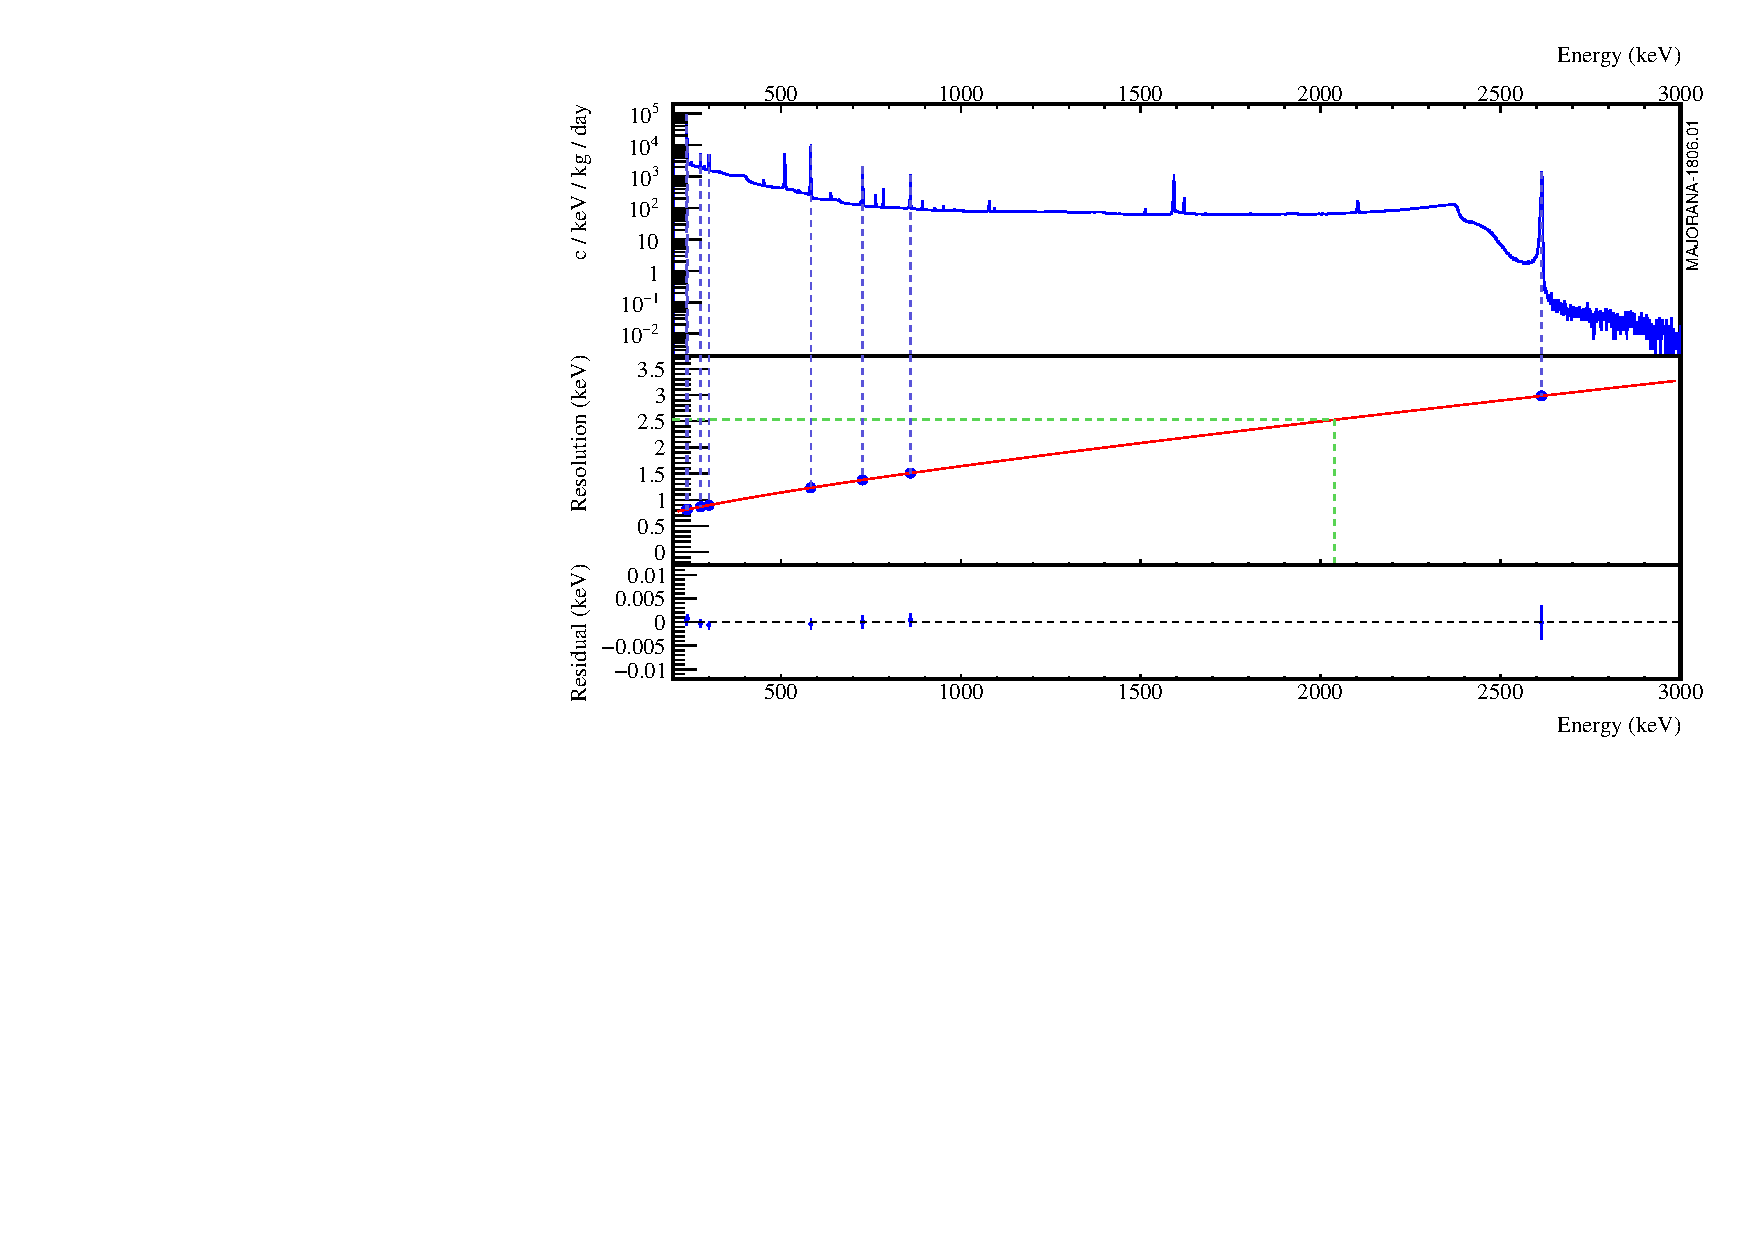
\includegraphics[width=.9\linewidth]{fwhmcal}
  \caption[FWHM extracted from a \Th{228} calibration spectrum]{\label{fig:fwhmcal}
    A \Th{228} calibration run with the FWHM fit curve and individual uncertainties at several peaks. This curve is used to compute the FWHM for a peak at a given energy. The statistical uncertainties is extracted from the fit result. An additional uncertainty is added to account for the uncertainties in the individual peaks; this is used to measure the uncertainty from energy nonlinearity.
  }
\end{figure}
\\
\subsection{Signal ROI Optimization}
The signal region of interest around each peak is optimized based on the peak shape functions as fit for each data set.
The signal region of interest is optimized following the procedure laid out in appendix~\ref{app:sens} and maximizing the rate sensitivity with respect to the region of interest upper and lower boundaries, $E_{low}$ and $E_{high}$ respectively.
\begin{equation}
  \hat\Gamma(E_{low}, E_{high}, \overline B) \propto \frac{\mathrm{DP}\big(\overline B(E_{high}-E_{low})\big)}{\epsilon_{ROI}(E_{low}, E_{high})}
\end{equation}
$\mathrm{DP}$ is the discovery potential as defined in appendix~\ref{app:sens}, where a flat background with background index $\overline B$ measured from data is assumed.
The efficiency is defined by the CDF of the Gaussian and LE tail components
\begin{equation}
  \label{eq:PDCDF}
  \begin{aligned}
    \epsilon_{ROI}(E_{low}, E_{high}; \mu, \sigma, f_{tail}, \tau) &= \frac{1}{2}\big(\mathrm{erfc}(\frac{E_{low}-\mu}{\sqrt{2}\sigma}) - \mathrm{erfc}(\frac{E_{high}-\mu}{\sqrt{2}\sigma})\big) \\& + f_{tail}\tau\big(\mathrm{ExGaus}(E_{high}; \mu, \sigma, \tau)-\mathrm{ExGaus}(E_{low}; \mu, \sigma, \tau)\big)
  \end{aligned}
\end{equation}
The optimal ROI is numerically calculated by minimizing $\frac{1}{\hat\Gamma(E_{low}, E_{high}, \overline B)}$ with respect to $E_{low}$ and $E_{high}$ using the minuit minimizer\cite{minuit}.
\\
\subsection{Background ROI Selection}
For each peak, a background ROI of width $50--100$~keV surrounding the peak is selected.
The ROI is selected to avoid any known background peaks and exclude them with at least $99.9\%$ efficiency.
A $99.9\%$ exclusion region calculated from the peakshape function is selected around the peak and removed from the background ROI.
\\
\subsection{ROI Detection Efficiency and Uncertainty} \label{sec:ROIEff}
The ROI detection efficiency is calculated from the CDF defined in equation~\ref{eq:PSCDF}.
The covariance matrix of the peak shape parameters obtained from the fit result is used to calculate the statistical uncertainty of the efficiency.
Several additional systematic effects must also be accounted for:
\begin{itemize}
\item \textbf{Gain drift:} \Th{228} energy calibrations are taken once per week, for 90 minutes each.
  In between these calibration runs, the energy calibration parameters undergo small adjustments that result in energy inaccuracies for background runs taken in between.
  This gain drift results in an increase in the width of the peak, which is accounted for by adding in quadrature $\sigma_{drift}$ to the value of $\sigma$ obtained from the fit.
  This also results in the dominant systematic uncertainty on the peak width, $\delta_{fwhm,drift}$.
  The gain drift also results in a small systematic error in the measured energy of the peak $\delta_{\mu,drift}$.
  A detailed description of the measurement of each of this systematic effect is contained in referece~\cite{energyunidoc}.  
\item \textbf{Energy nonlinearity:} While the energy response for HPGe detectors is ostensibly linear, several factors result in small nonlinearities.
  Local nonlinearities that are correlated over small energy scales of arise from the response of the Gretina digitizers.
  While these nonlinearities are corrected for, a nonlinearity of $\sim0.1$~keV with a period of $\sim300$~keV remains.
  Global nonlinearities result from systematic uncertainties in the energy estimation.
  One source of global nonlinearity arises from uncertainty in the start time of the waveform, which is energy dependant.
  Another is a small quadratic term resulting from charge recombination.
  Because calibrations are performed on peaks with energies ranging from 238~keV to 2614~keV, energy shifts due to global nonlinearities are very small in this range and local energy nonlinearities dominate.
  At smaller and larger anergies, the shifts can be as large as $\sim0.5$~keV in some detectors.
  Energy nonlinearities result in an increase in $\sigma$ as a result of the combining of peaks with different shifts; however, since the energy calibrations include all detectors, this shift is already included in the fit result, so no action is required.
  Energy nonlinearities also have a significant affect on the uncertainty in the measured peak energy, $\delta_{\mu,NL}$, which is a dominant uncertainty.
  A detailed description of the measurement of each of this systematic effect is contained in referece~\cite{energyunidoc}.
\item \textbf{Detector Crosstalk:} Because we are searching for peaks in coincidence events, the possibility for a distortion in the energy measurement due to crosstalk between the involved events exists.
  This effect is measured in section~\ref{sec:crosstalk} to be small enough that no energy correction or peakshape correction is required.
  However, this effect does contribute to small uncertainties in the peak position, $\delta_{\mu,xtalk}$ and peak width, $\delta_{fwhm,xtalk}$.
\end{itemize}

Once these uncertainties have been measured, they must be propagated into the detection efficiency.
The statistical and systematic uncertainties on $\mu$ and the FWHM are added in quadrature to obtain $\delta_\mu$ and $\delta_{fwhm}$.
The uncertainty on the FWHM is used to calculate a width scale uncertainty, $\delta_\alpha$, which is simply the fractional uncertainty on the FWHM.
To compute the uncertainty on the efficiency, the efficiency is computed after modifying the peakshape parameters by one-sigma in either direction.
For the uncertainty from the width, we take:
\begin{equation}
  \begin{aligned}
    \sigma_{\epsilon_{ROI},fwhm} &= \frac{1}{2}\big(\epsilon_{ROI}(E_{low}, E_{high}; \mu, \sigma(1+\delta_\alpha), f_{LE}, \tau(1+\delta_\alpha)) \\&+ \epsilon_{ROI}(E_{low}, E_{high}; \mu, \sigma(1-\delta_\alpha), f_{LE}, \tau(1-\delta_\alpha))\big)
  \end{aligned}
\end{equation}
Because the ROI is optimized to around $\mu$, shifts in the peak in either direction will cause a reduction in efficiency; for this reason, we must perform a second order propagation of uncertainties.
The result is a slight degradation in the efficiency, so that
\begin{equation}
  \epsilon_{ROI} =  \frac{\epsilon_{ROI}(E_{low}, E_{high}; \mu + \delta_\mu, \sigma, f_{LE}, \tau) + \epsilon_{ROI}(E_{low}, E_{high}; \mu - \delta_\mu, \sigma, f_{LE}, \tau)}{2}
\end{equation}
and
\begin{equation}
  \sigma_{\epsilon_{ROI},\mu} = \epsilon_{ROI}(E_{low}, E_{high}; \mu) - \epsilon_{ROI}
\end{equation}
These uncertainties are taken to be uncorrelated and added in quadrature to obtain the final uncertainty on the ROI efficiency.
Table~\ref{tab:energysystematics} contains a full summary of all of the energy uncertainties, the ROIs, and the ROI efficiencies and uncertainties.
\begin{sidewaystable}[p]
  \caption[Energy systematics]{ \label{tab:energysystematics}
    Table of energy estimation uncertainties, regions of interest, and efficiencies
  }
  \resizebox{\textwidth}{!}{%
  ../../appAllResults/tables/table_2vBB_ES0_1_pseff.tex }
\end{sidewaystable}

\subsection{Detector Crosstalk}
Detector crosstalk is caused when a true signal in one detector channel induces a small signal in another channel.
This is not a large enough evect to trigger events in a separate channel, meaning that it does not effect \ss\ events.
However, it could produce an energy estimation error in \md\ events since coincident pulses could induce signals that interfere either constructively or destructively, shifting the measured energy.
In practice, this could produce both a shift and additional uncertainty in both the measured energy of the peak and in the width of the peak.
To check for this effect, we can look at \md\ events in \Th{228} calibration data.
In particular, we will compare the centroid and FWHM for several peaks in both \sd\ events and \md\ events.
\begin{figure}[p]
  \centering
  \subfloat[Module 1]{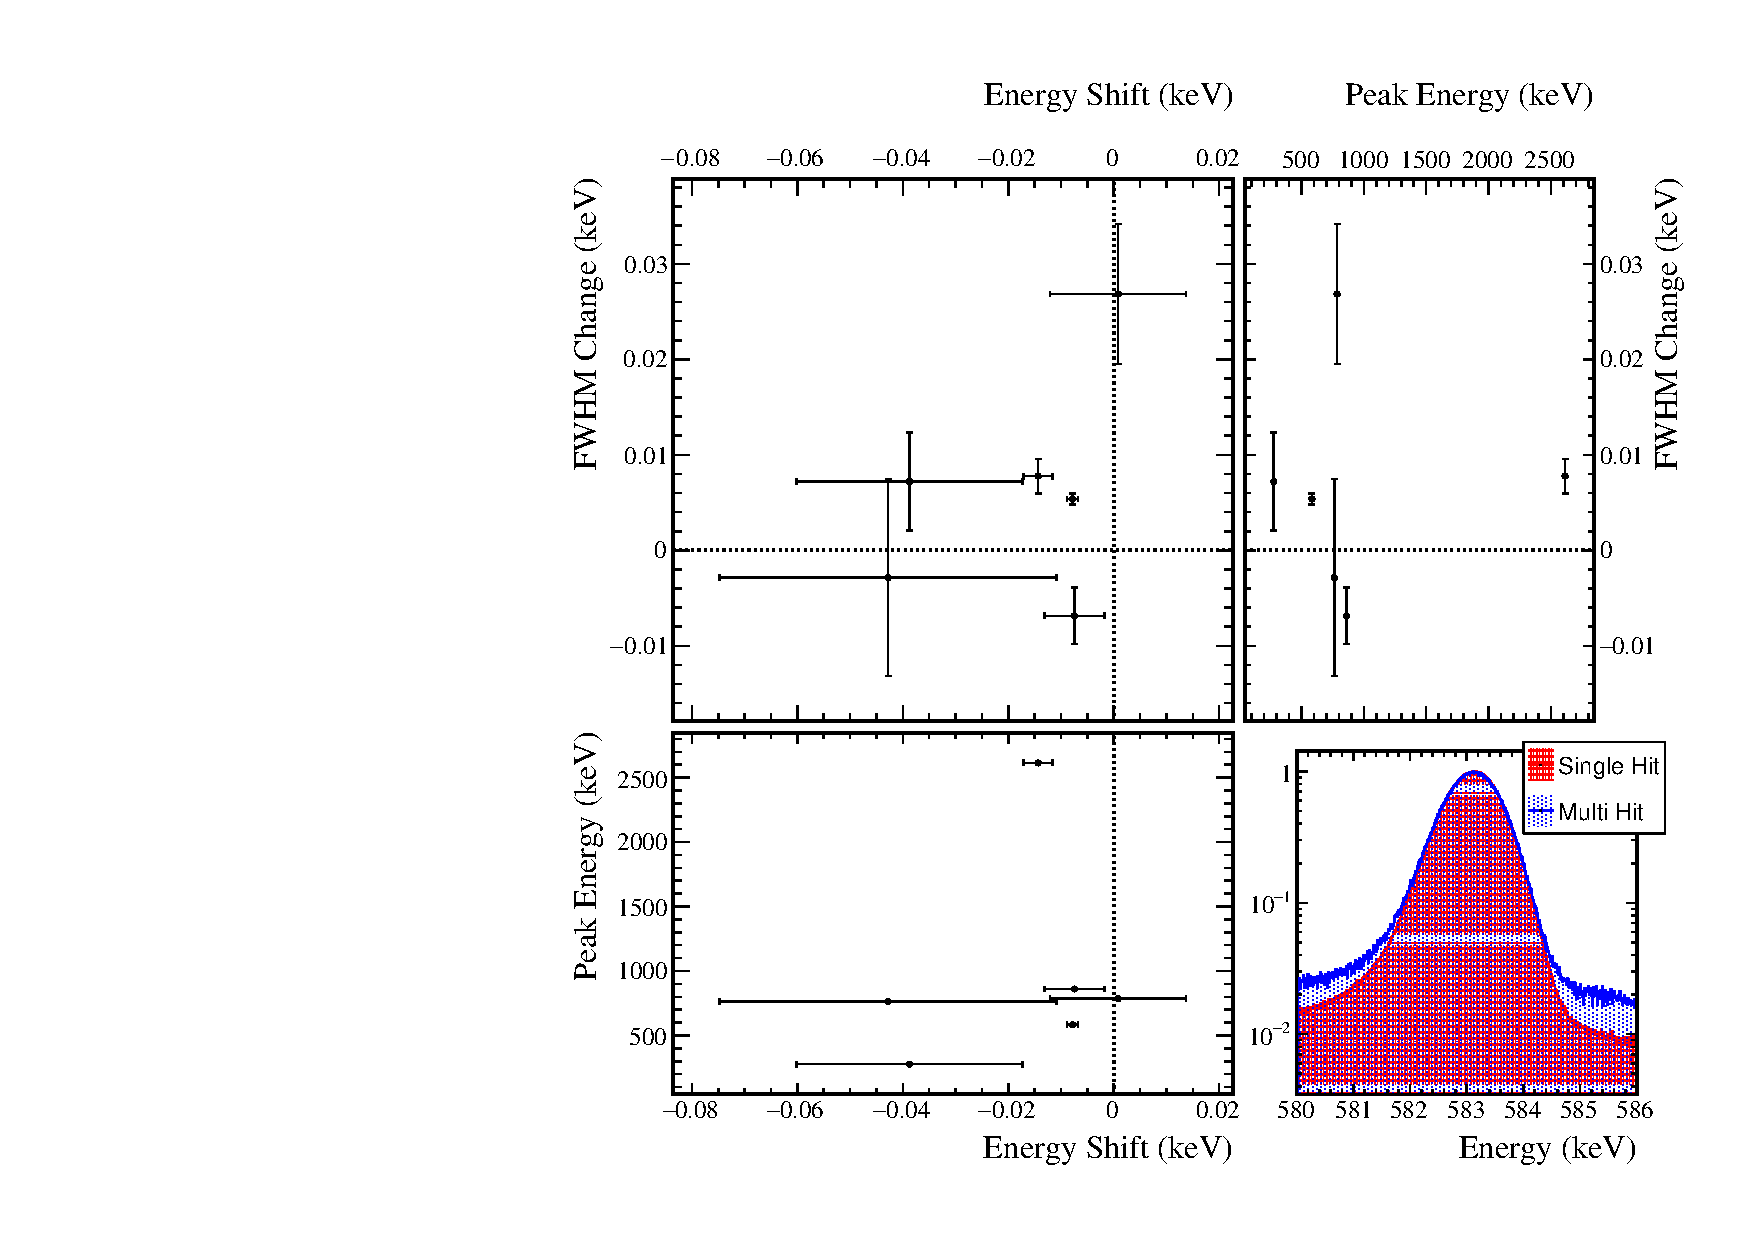
\includegraphics[width=\linewidth]{xtalkplot}}
  \caption[Peak shape comparison for single- and multi-detector events]{\label{fig:xtalk}
    Difference of the measured centroid and FWHM of several \Th{228} calibration peaks. Error bars represent the fit errors. Notice on the bottom right, that any difference is not visible to the naked eye.
  }
\end{figure}
\\
5 peaks were selected from the \Tl{208} $\gamma$ cascade, at 277, 583, 763, 860 and 2614~keV, and one additional peak was selected from the \Bi{212} cascade, at 785~keV.
The combined calibration spectra from dataset~6 were used to perform this analysis.
These peaks were fit individually, and the centroid and FWHM were computed for multiplicity 1~and multiplicity~2 events.
Figure~\ref{fig:xtalk} shows the results of these measurements.
While a very small reduction in peak centroid and increase in peak width are observed, the shifts are small compared to the existing uncertainties in these parameters.
As a result, we will ignore this shift and instead compute an uncertainty in each parameter caused by crosstalk.
We will treat the systematic error as uncorrelated between the peaks and compute the necessary error needed to make the combined statistical and systematic errors large enough to make the $\chi^2$ value computed by comparing these peaks equal to 1:
\begin{equation}
  \chi^2 = \displaystyle\sum_{k=0}^N \frac{(\mathrm{cen}_{k,m1} - \mathrm{cen}_{k,m2})^2}{\sigma_{cen,k,m1}^2+\sigma_{cen,k,m2}^2+\delta_{\mu,xtalk}^2}
\end{equation}
\begin{equation}
  \chi^2 = \displaystyle\sum_{k=0}^N \frac{(\mathrm{FWHM}_{k,m1} - \mathrm{FWHM}_{k,m2})^2}{\sigma_{fwhm,k,m1}^2+\sigma_{fwhm,k,m2}^2+\delta_{fwhm,xtalk}^2}
\end{equation}
Both systematic errors are numerically computed using a Brent minimization algorithm.
The results are $\delta_{\mu,xtalk}=0.012$~keV and $delta_{fwhm,xtalk}=0.011$~keV, both of which are subdominant uncertainties.


\section{Background Cuts}
By making use of known properties of background events, data cleaning cuts can be designed to selectively reduce backgrounds while minimizing sacrifice of excited state events.
Because of the \md\ nature of the event selection, many of these background cuts are designed that make use of observables from the detector hits in coincidence with candidate hits.

\subsection{Enriched Source Detector Cut}
Since the \bbes\ events must originate in \Ge{76}, events are far likelier to originate in enriched Germanium detectors than those with natural Germanium isotopic abundances.
There are 29.8~kg of enriched detectors, with $88.1 \pm 0.7$\% abundance of \Ge{76} and 14.4~kg of natural detectors, with $7.83 \pm 0.07$\% abundance of \Ge{76}.
This means that $95.8 \pm 0.1$\% of \bbes\ events will originate in enriched detectors.
If we assume that background events will hit all detector mass at the same rate, then we would expect only 67\% of hits from background events involving two detectors to be in coincidence with a hit in an enriched detector.
This means that a significant gain in sensitivity can be acheived by cutting hits that are not in coincidence with an enriched detector hit.
While the detection efficiency of this cut is expected to be close to 95.8\%, the actual efficiency is measured from simulations, and tends to be greater, since a greater proportion of enriched detectors are active than of natural detectors.

\begin{figure}[h]
  \centering
  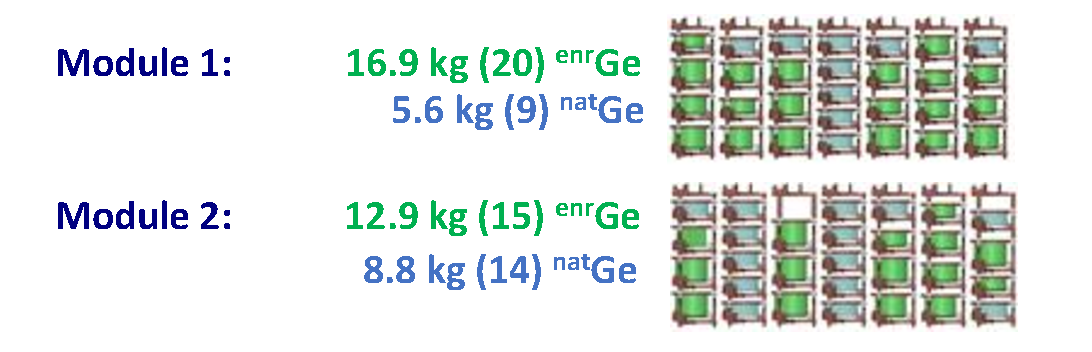
\includegraphics[width=0.8\textwidth]{enrnatdets}
  \caption[Module 1 and Module 2 enriched and natural detectors]{\label{fig:Ge76BBLevelDiagram}
    Diagram showing each detector in each module, arranged by which string and position they are in. Enriched detectors are colored green and natural detectors are colored blue. 95\% of \Ge{76} is contained in the enriched detectors.}
\end{figure}

\subsection{Coincident and Sum Energy Cuts} \label{sec:MSenergycuts}
The greatest source of background events is expected to be $\gamma$-rays from a handful of known primordial and cosmogenic isotopes.
Because $\gamma$ photons are monoenergetic, these backgrounds will often present a clear detection signature that can be targetted.
$\gamma$ photons will often Compton scatter from one detector into another, depositing their entire energy between the two.
For this reason, events whose total energy is equal to the energy of a known $\gamma$ can be cut.
$\beta$-decays will often result in a cascade of multiple $\gamma$s, at least one of which may be fully absorbed in a single detector.
These events can be cut by searching for a coincident detector with energy equal to that of a known $\gamma$.
Finally, whereas the \bb\ decay spectrum approaches zero amplitude at low energies and at \Qbb, the Compton continuum of $\gamma$s has finite amplitude at low energies.
This means that sensitivity can be gained by setting low- and high-energie thresholds on hits in coincidence with a candidate event.
These combined backgrounds can be reduced by cutting events with either sum energies or coincident hit energies that fall in a set of energy ranges.
For \bbes\ modes with multiple $\gamma$s, the expected energy ranges will vary differ in natural and enriched detectors, since natural detectors will mostly include hits from one of the $\gamma$s, while enriched events will include \bb\ hits, $\gamma$ hits, and pileup events including both of these, allowing a much wider energy range.
For this reason, a separate set of coincident cut energy ranges are found for natural and enriched detectors.
\\
The energy ranges that are cut can be determined by comparing the background model simulation to simulations of each \bbes\ decay mode.
An algorithm was written that simultaneously selects a set of both sum and coincident energy ranges to cut that optimizes discovery potential, as described in appendix~\ref{app:sens}.
The algorithm begins by identifying events in the \bbes\ simulation that include at least one hit consisting of the full absorption of a $\gamma$ photon and events in the background model simulation that include at least one hit in the background region of interest.
These events are then sorted into energy bins for each coincident hit and for the sum energy of the event (a single event will be in multiple bins).
For each bin, the algorithm checks the change in discovery potential if the bin was toggled to be either cut or readded.
Following equation~\ref{eq:cutcriterion}, the discovery potential will be improved for bin $k$ if:
\begin{equation}
  \mathrm{DP}'(s\cdot N_{BG})\frac{s\cdot n_{k,BG}}{\mathrm{DP}(s\cdot N_{BG})} < \frac{n_{k,ES}}{N_{ES}}
\end{equation}
where $N_{ES}$ and $N_{BG}$ are the total number of events remaining in the simulated \bbes\ and background spectra, respectively, $s$ is a scaling to estimate the number of background events in the data from the number in the simulation, and $n_{k,ES}$ and $N_{k,BG}$ are the number of simulated \bbes\ and background events contained in the bin.
A $\chi$ value is computed representing the normal quadrile of the probability that cutting or readding the bin will improve the discovery potential.
This is done by assuming that the uncertainty on the number of events in the bin is Gaussian distributed, with standard deviations $\sqrt{n_{k,ES}}$ and $\sqrt{n_{k,BG}}$, respectively.
In this case, we get:
\begin{equation}
  \chi_k = \frac{ \frac{n_{k,ES}}{N_{ES}} - \mathrm{DP}'(s\cdot N_{BG})\frac{s\cdot n_{k,BG}}{\mathrm{DP}(s\cdot N_{BG})} }{ \sqrt{ (\mathrm{DP}'(s\cdot N_{BG})\frac{s}{\mathrm{DP}(s\cdot N_{BG})})^2n_{k,BG} + \frac{n_{k,ES}}{N_{ES}^2} } }
\end{equation}
All events in the bin with highest probability of improving the discovery potential are then either cut or readded, and must be cut or readded to all other bins that they fall into.
Note that a readded event will only be readded if it is not cut by any other bin.
This process is repeated until toggling any bin will have $\chi_k<0$, meaning there is a $<50$\% chance of improving the discovery potential.
At this point, the bins are then combined in order to determine the ranges of energies to be cut in sum energy and coincident energies.
\\
Because of limited statistics in the simulations, this cut will be biased to cut events with a downward fluctuation in \bbes\ amplitude and accept bins with an upward fluctuation in \bbes\ amplitude, and vice-versa for the background model.
In order to minimize this bias and ensure that energy ranges are selected based on real backgrounds rather than statistical fluctuations, a penalty is applied to the probability calculations if a new range would be added.
If a cutting or readding a bin would increase the number of energy ranges, a penalty of 3 is added to the $\chi$ value, and if it would reduce the number of ranges, a penalty of -3 is added.
This corresponds to requiring a 99.8\% chance that adding a new energy range will represent an improvement before we conclude that it is not a statistical fluctuation.
This is inspired by the Akaike Information Criterion (AIC), which adds a penalty of 1 to a likelihood for each parameter added to a model.
In this case, adding an energy range adds two parameters to our cut, so the equivalent penalty is 1.5 per parameter, which is a larger penalty than AIC.
\\
To further control limited simulation statistics, a variety of bin widths is used to determine the optimal energy ranges.
This is necessary because with a narrow binning, bins do not have enough statistics to overcome the penalty described above, but wider bins produce very imprecise energy ranges.
The algorithm starts by optimizing the cut ranges with a bin width of 6.4~keV starting from a prior of cutting no energy ranges.
Once this optimization is complete, the bin width is split in half and the algorithm re-optimizes the energy ranges, using the previous ranges as a prior.
This halving of bin width is repeated until a final bin width of 0.2~keV is reached.
The results of this cut optimization procedure are shown in figures~\ref{fig:sumandcoinEcuts} and~\ref{fig:2Dcuts}.
\\
\begin{figure}[!h]
  \centering
  \subfloat[Simulated BG Sum Energy Spectrum]{\includegraphics[width=.5\linewidth]{BGSumECut}}
  \subfloat[Simulated ES Sum Energy Spectrum]{\includegraphics[width=.5\linewidth]{ESSumECut}}\\
  \subfloat[Simulated BG Coincident Energy Spectrum]{\includegraphics[width=.5\linewidth]{BGCoinECut}}
  \subfloat[Simulated ES Coincident Energy Spectrum]{\includegraphics[width=.5\linewidth]{ESCoinECut}}
  \caption[Sum and coincident simulated energy spectra with cuts]{\label{fig:sumandcoinEcuts}
    Top: Sum energy spectra of simulated ES and BG events. The events in red are cut by the sum- or coincident-energy cut. Note that the region around many peaks is cut out. This is the intdended effect of the sum energy cut.\\
    Bottom: Energy spectrum of events in coincident with events in the ROI. Events in red are cut by the sum- or coincident-energy cut. Once again, regions around prominent peaks are cut out as intended.
  }
\end{figure}

\begin{figure}[h]
  \centering
  \includegraphics[width=0.8\linewidth]{BG2Dcuts}
  \caption[2D energy spectrum of simulated BG events]{\label{fig:2Dcuts}
    2D energy spectrum of simulated BG events. Blue bins have at least one hit that passes both the sum- or coincident-energy cuts. For red bins, both hits have failed at least one of these cuts. Green bins have at least one hit in the BG or ES ROI that passes these cuts.
    }
\end{figure}

\begin{figure}[h]
  \centering
  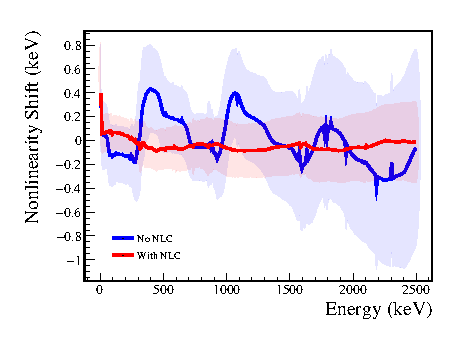
\includegraphics[width=0.8\linewidth]{DigitizerNonlinearity}
  \caption[Measured Digitizer Nonlinearity vs Energy]{\label{fig:dignonlin}
    Digitizer nonlinearity before (red) and after (blue) begin corrected. This nonlinearity is measured by comparing the energy measured in the high gain channel to that of the low gain channel.
  }
\end{figure}
The application of the sum and coincident energy cuts will introduce systematic error to the efficiency measurement.
For the \tnbb\ decay modes, the coincidence events will have a broad energy spectrum, so the systematic error will be dominated by errors in that spectrum or in the energy estimation.
Since the efficiency is calculated by integrating over portions of the coincidence spectrum, an upper limit on the systematic error can be found using the KS statistic of a comparison between the simulated spectrum and the true spectrum.
As discussed in section~\ref{decay0}, we can compare the decay0 simulated spectrum to the true spectrum using the Iachello simulated spectrum.
To account for energy nonlinearity, each energy is shifted to represent the effects of digitizer nonlinearity and energy drift.
Digitizer nonlinearity originates from the fact that some digitizer energy bins are slightly wider than others and has an approximately sawtooth dependency on energy with a period of $\sim600$~keV.
A correction is applied that reduces the size of of this nonlinearity to $\sim0.1$~keV in magnitude and smooths it out significantly, as shown in figure~\ref{fig:dignonlin}.
Digitizer nonlinearity is corrected by shifting each energy according to a sawtooth function with rms 0.1~keV and period 600~keV:
\begin{equation}
  \Delta(E) = \sqrt(3)\cdot (0.1~\mathrm{keV}) \big(\mathrm{rem}(\frac{E-150~\mathrm{keV}}{600~\mathrm{keV}}) \big)
\end{equation}
where $\mathrm{rem}$ is the remainder function as defined in the \cpp standard library.
An additional shift that is randomly sampled from a Gaussian distribution with standard deviation $0.00015\cdot E$ is applied to simulate the effect of gain drift, based on the drift observed during DS5.
After applying both of these corrections to the decay0 spectrum, a KS test is performed against the Iachello spectrum, and a KS statistic of 0.08\% is observed, as shown in figure~\ref{fig:decay0NLCks}.
This statistic is used as an upper limit on the uncertainty from the energy range cuts for \tnbb modes.
\begin{figure}[h]
  \centering
  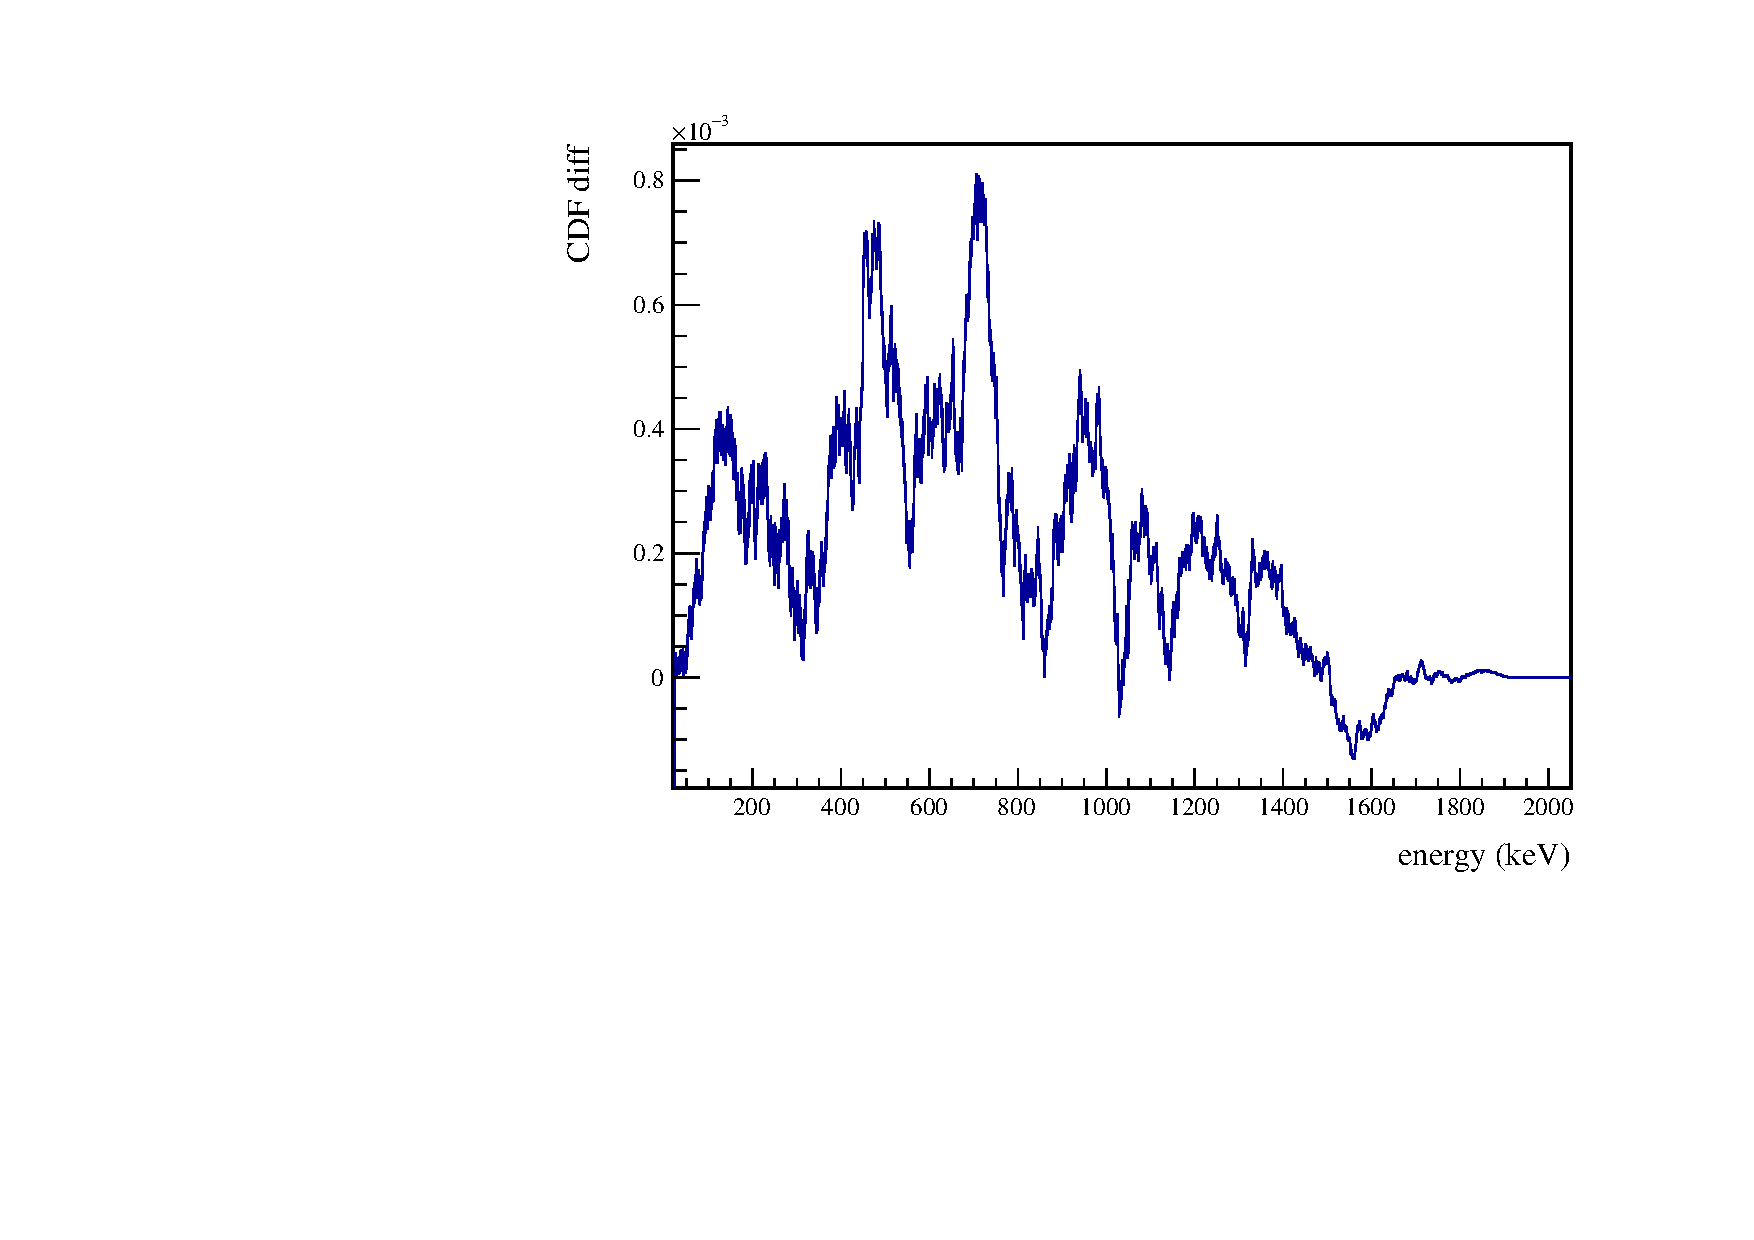
\includegraphics[width=0.6\linewidth]{decay0KS}
  \caption[KS Test of decay0 spectrum with energy non-linearities vs Iachello spectrum]{\label{fig:decay0NLCks}
    KS test comparing the simulated decay0 \tnbb\ ground state decay with energy nonlinearities applied to the simulated spectrum using the Iachello phase space factors.
  }
\end{figure}
\\
For \znbb, the energy ranges selected by this cut tend to surround peaks corresponding to the \Qbb s of the decay modes.
In this case, since we are no longer integrating over a \bb -spectrum, the uncertainty in the efficiency will depend on shifts in the peak, similar to the ROI-efficiency.
Since the energy regions selected keep at least 99.9\% of these peaks in all cases, we can set an upper limit on the uncertainty by checking the ROI efficiency uncertainty around the 2039~keV \Qbb, assuming an ROI tuned to select 99.9\% of the peak.
The uncertainty observed in this case is 0.325\%, which is applied to the energy range cuts for \znbb modes.
For both \znbb\ and \tnbb\ modes, this efficiency uncertainty is sub-dominant, so these upper limits will suffice.
\\
\subsection{Muon Veto Cut}

\begin{figure}[ht]
  \centering
  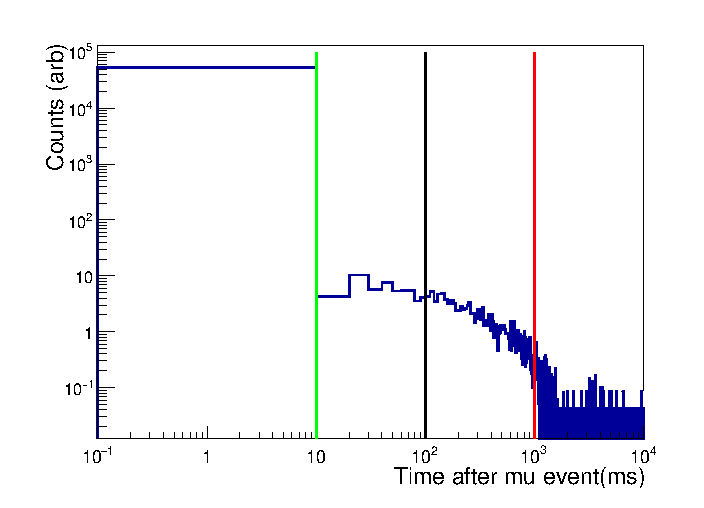
\includegraphics[width=0.8\textwidth]{muvetoeff}
  \caption[Simulated efficiency of muon veto cut]{\label{fig:muvetoeff}
    A histogram of muon-induced Germanium detector events based on their delay after their detection by the muon veto system. A cut of 1~s after the veto time will remove $>99.9$\% of muon-induced events.\cite{2015wiseman}}
\end{figure}

Cosmic ray muons have the potential to produce partical showers in the \MJD\ that can produce \msmd\ events and can activate short-lived isotopes that in turn may decay, producing delayed \msmd\ events.
Background events caused by muons can be cut using the muon veto system described in section~\ref{sec:muveto} \cite{2015wiseman}.
If a muon passes through the \MJD\, it must pass through two surfaces of the muon veto panels.
Any time veto panels from at least two different surfaces simultaneously measure events above a certain energy threshold, we assume that event was a muon.
Any Germanium detector events for the next 1~s after the muon event are then cut.
This cut will remove $>99.9$\% of events induced by the muon shower, based on simulations shown in figure~\ref{fig:mucut}.
In reality, the cut efficiency is slightly lower due to periods of time where the muon veto system clock became desynchronized with the Germanium detector clock.
The impact of this cut is to reduce the total livetime by $<40$~s per day.
\\
\section{Final Efficiency Measurements}
The final efficiency measurement combining all of the effects described in this chapter for each \bbes\ mode is measured directly from the simulations.
The efficiency used is the average of the simulated efficiency for each subdataset, weighted by the exposure of that subdataset.
Because each module is an independant measurement, separate efficiencies are measured for modules~1 and~2.
Because of correlations causing the probability of certain effects causing sacrifice of a \bbes\ event to be conditional on other effects, the combined efficiency will differ from simply being the product of the individual efficiencies.
This means that the combined efficiency $\epsilon_{comb}$ for each effect $k$ is:
\begin{equation}
  \epsilon_{comb} = \prod_{k=0}^N P(\mathrm{event~is~cut} | \mathrm{cuts~} 0\dots k-1 \mathrm{~are~applied})
\end{equation}
In spite of this, we will assume that the sources of error are uncorrelated and the fractional uncertainty is independant of what other effects have been applied.
This implies that the uncertainty on the combined efficiency, $\sigma_{\epsilon,comb}$ can be expressed as:
\begin{equation}
  \sigma_{\epsilon,comb}=\epsilon_{comb} \sqrt{ \sum_{k=0}{N} (\frac{\sigma_{\epsilon,k}}{\epsilon_k})^2 }
\end{equation}
The values $\epsilon_k$ represent the probability of cutting an event assuming all other cuts are applied.
Table~\ref{tab:eff_2vBB_0_1} shows the efficiency for each effect described in this chapter and uncertainty on each efficiency, and the combined efficiency and uncertainty.
\begin{table}[h]
  \centering
  ../../appAllResults/tables/table_2vBB_ES0_1_efficiency.tex
  \caption[Detection efficiency summary for \tnbb\ to the \SP{0}{+}{1} state of \Se{76}]{\label{tab:eff_2vBB_0_1}
    Table of detection efficiencies and uncertainties for \tnbb\ of \Ge{76} to the \SP{0}{+}{1} state of \Se{76}. Note that the efficiencies are the combined efficiency for the 559 and 563~keV peaks.
  }
\end{table}
Similar tables for each other \bbes\ peak are shown in appendix~\ref{app:allresults}.
In all cases the dominant uncertainties come from either the dead layer thickness or the simulation uncertainty.
Figure~\ref{fig:escuteffects} shows the effect of each cut as it is applied sequantially to the \tnbb\ to \SP{0}{+}{1} peaks.
\begin{figure}[htb]
  \centering
  \includegraphics[width=0.8\textwidth]{ESAllcuts}
  \caption[Simulated \tnbb to \SP{0}{+}{1} peaks with cuts applied]{\label{fig:escuteffects}
    The 559~and 563~keV peaks from the \tnbb\ decay to the \SP{0}{+}{1} decay mode, with the effect of all cuts applied sequentially to simulated ES events. The cuts are applied from top to bottom (i.e. red, blue, then green). Many events will be cut by more than one of these; in that case it will be colored by whichever cut is applied first. 
  }
\end{figure}

\end{document}